\documentclass[thesis.tex]{subfiles}

\begin{document}

\chapter{Evaluation}\label{chap:eva}
This chapter will evaluate the proposed algorithms both from a performance and a quality perspective.
In the last section we try to compare our technique to related works.
However, as we were not able to implement comparable implementations within the bounds of this project, we can only provide comparisons on an abstract level.

\section{Test Setup \& Scenes} \label{sec:eva:setup}
All tests were rendered using a Nvidia GTX670 desktop graphics card.
The test machine contains an Intel i7-3770 CPU and uses Windows 8.1 64bit as OS.

\begin{figure}
\centering
\begin{subfigure}[b]{0.8\textwidth}
\centering
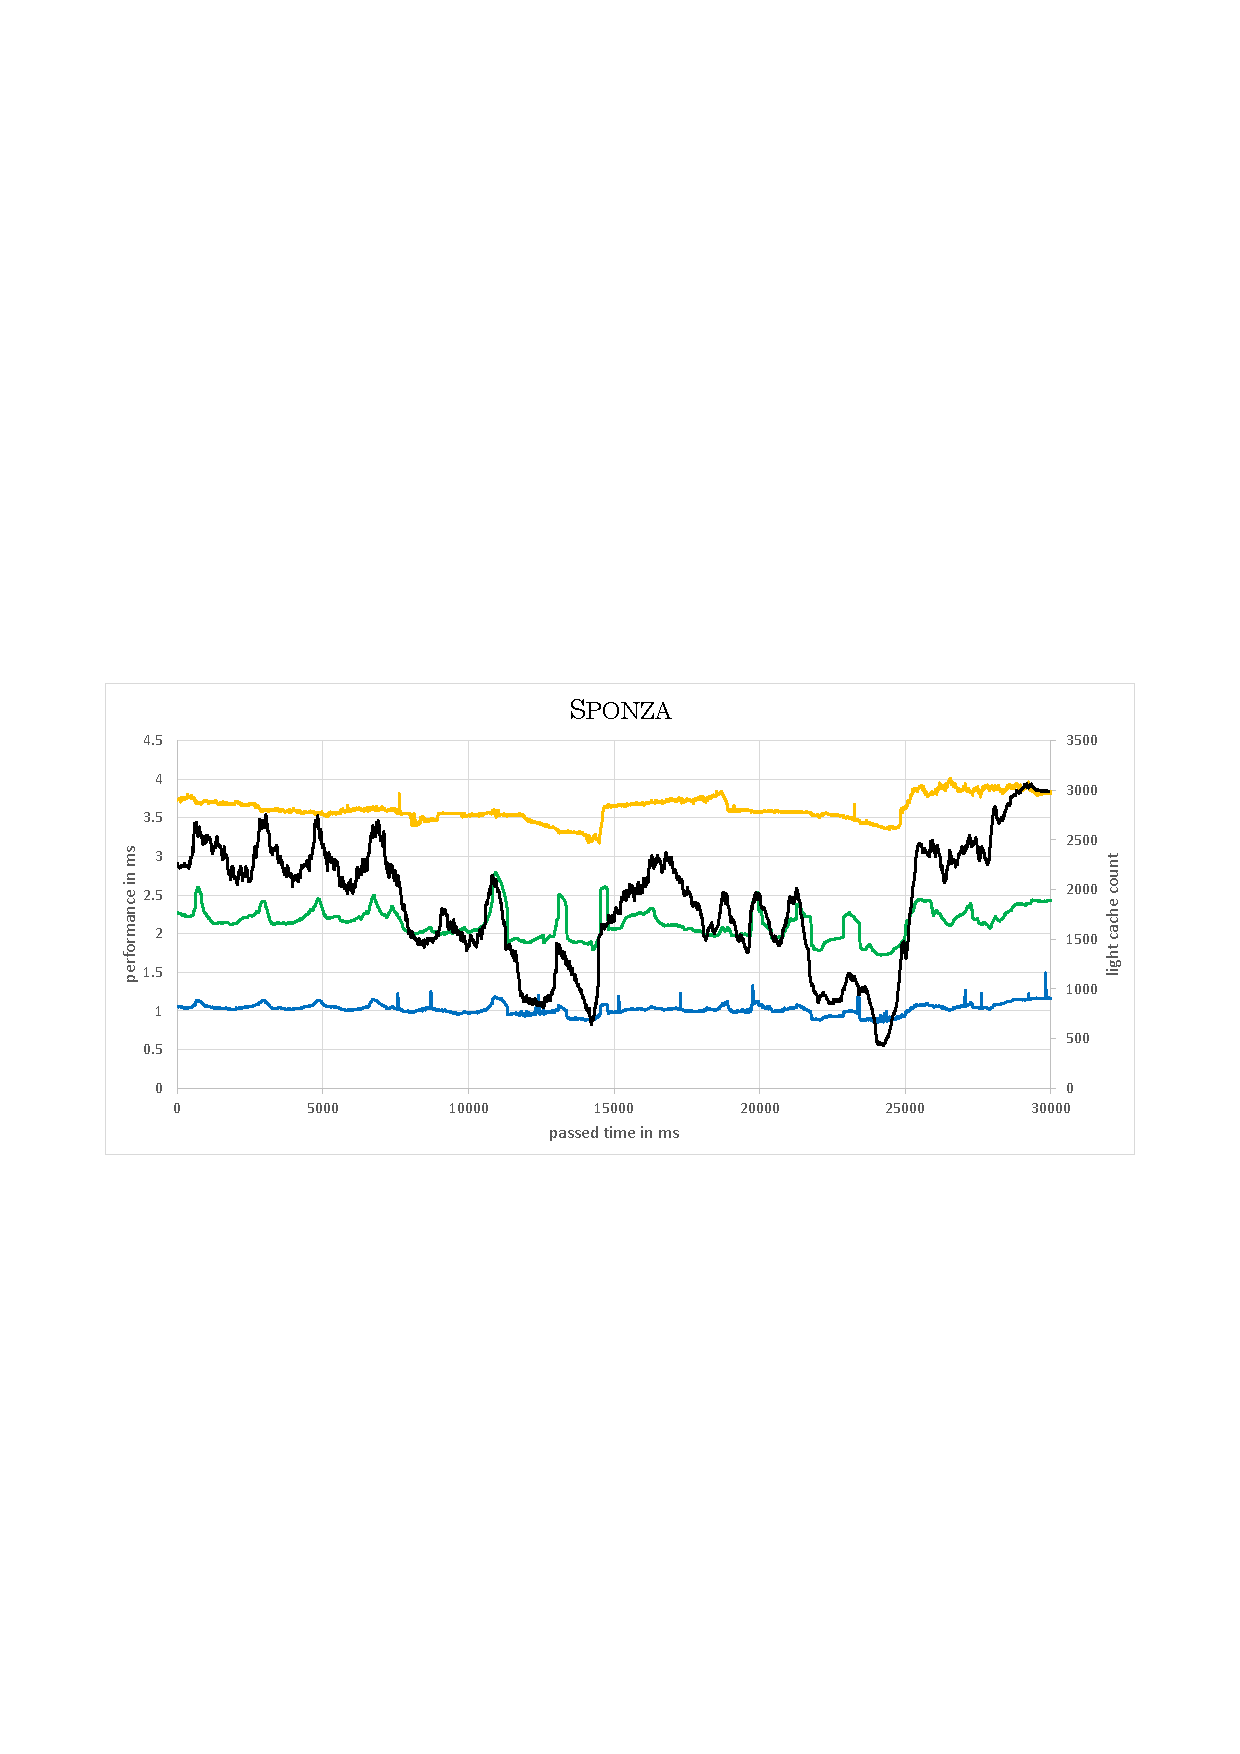
\includegraphics[width=\textwidth]{eva/scenes/sponza}
\caption{\dataset{Sponza}}
\end{subfigure}
\\
\begin{subfigure}[b]{0.8\textwidth}
\centering
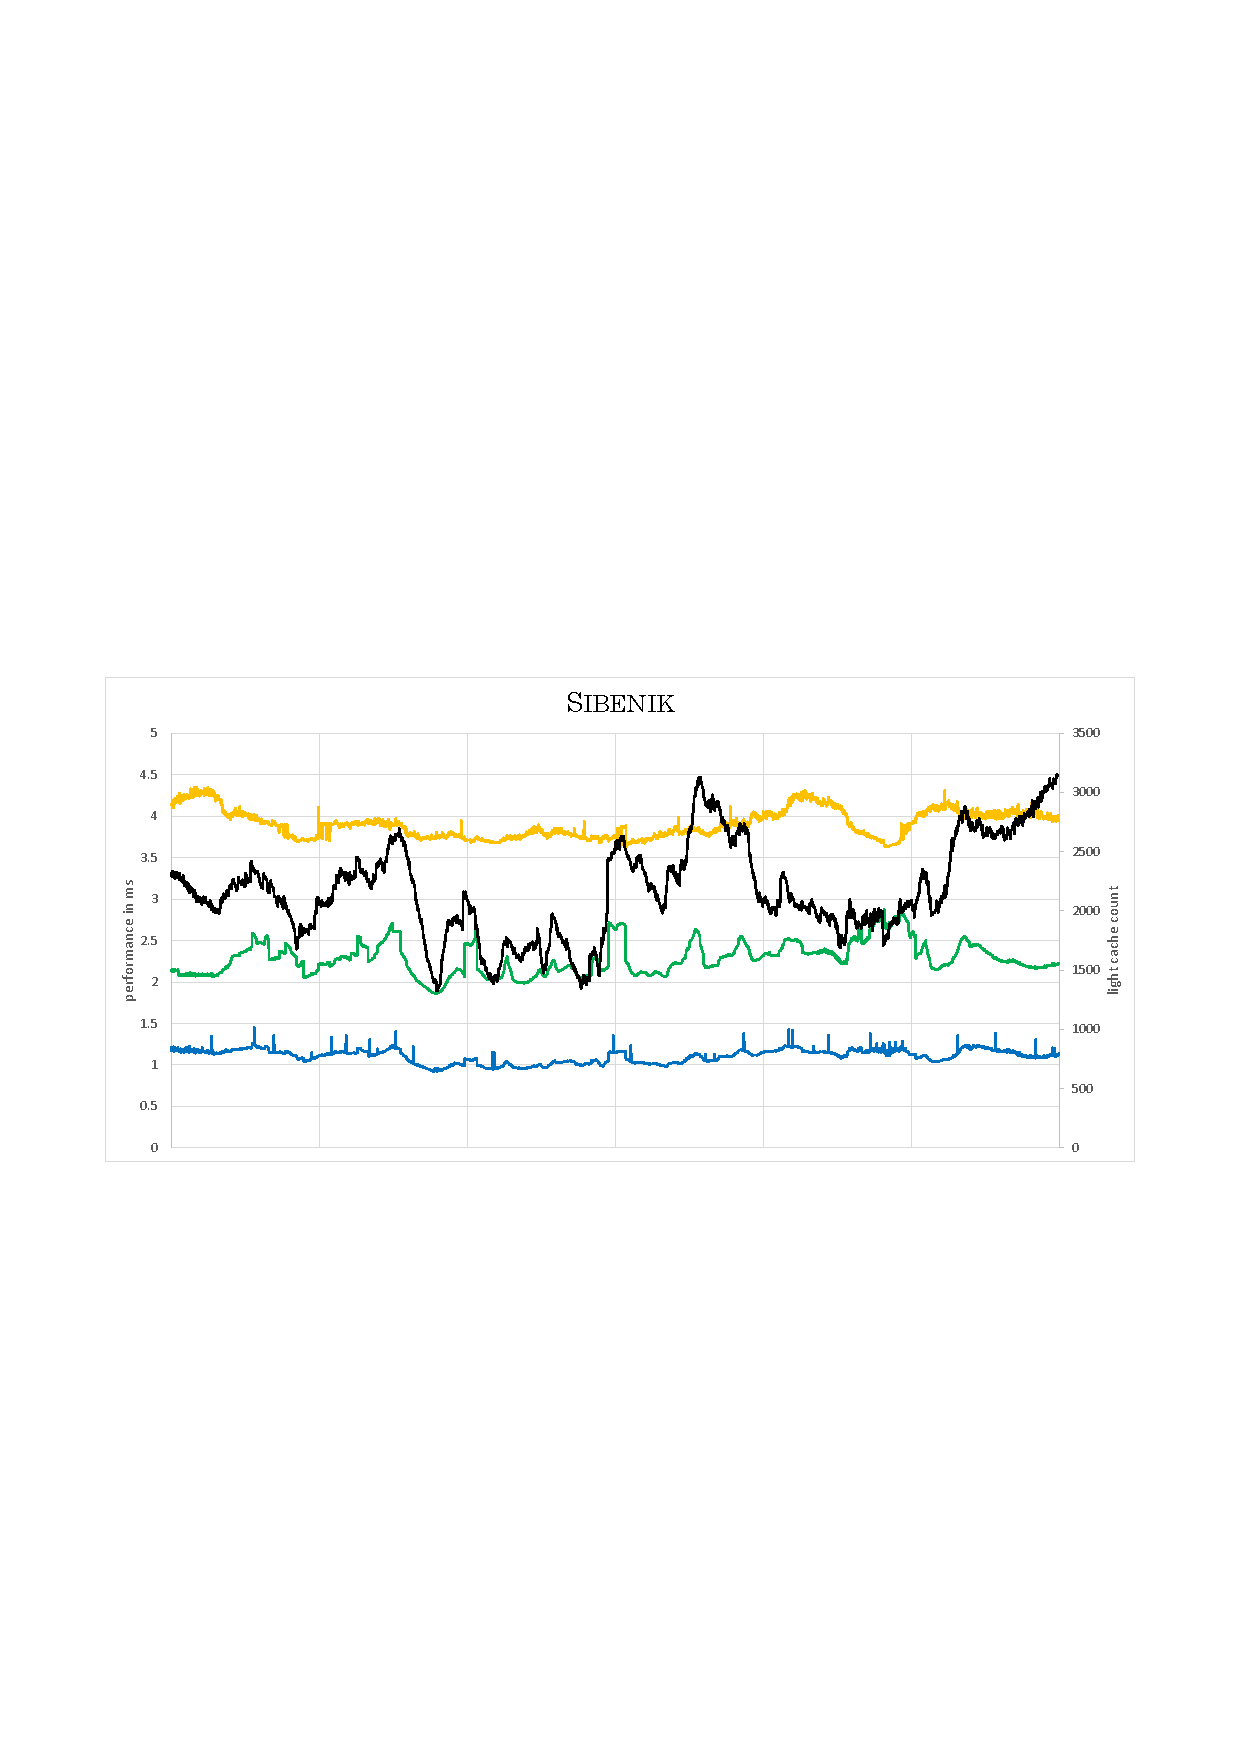
\includegraphics[width=\textwidth]{eva/scenes/sibenik}
\caption{\dataset{Sibenik}}
\end{subfigure}
\\
\begin{subfigure}[b]{0.8\textwidth}
\centering
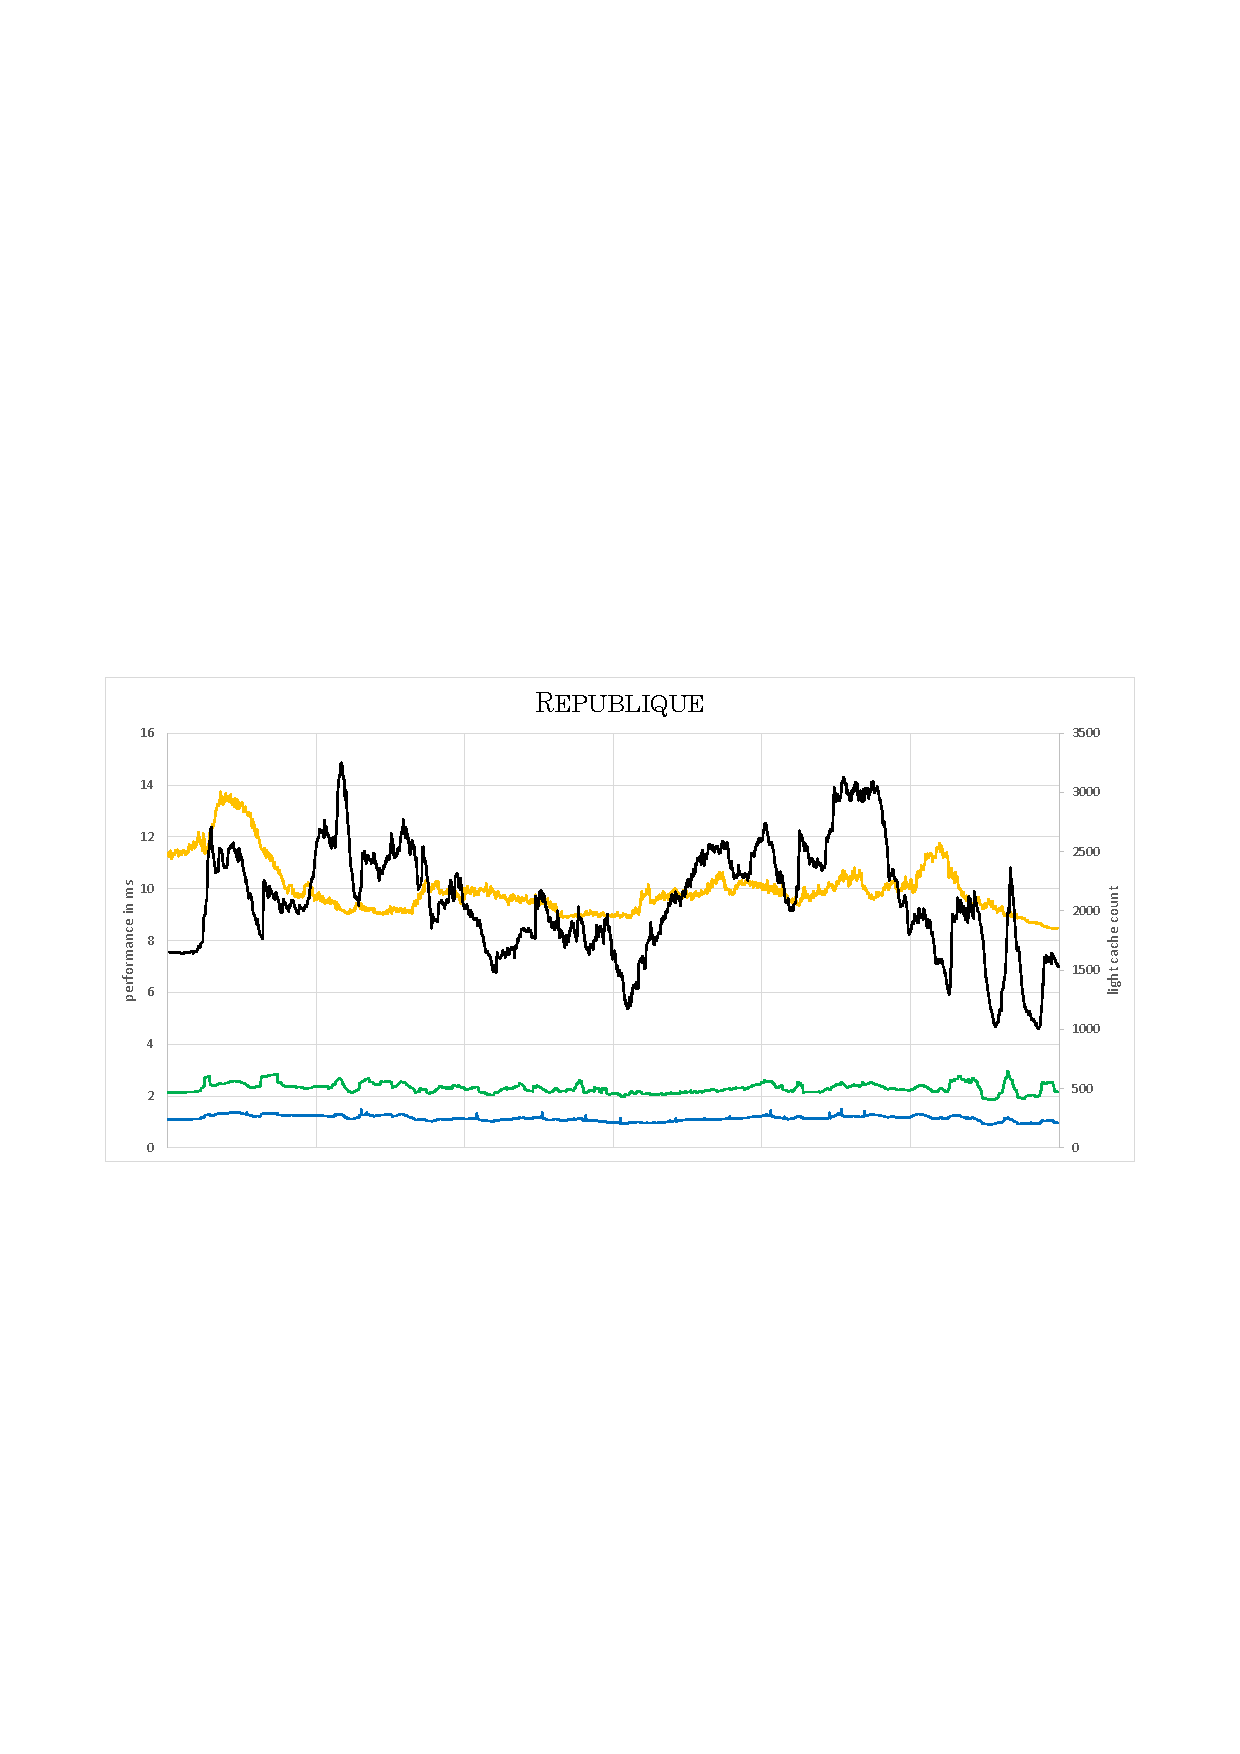
\includegraphics[width=\textwidth]{eva/scenes/republique}
\caption{\dataset{Republique}}
\end{subfigure}
\caption{Overview over our three main test scenes.}
\label{fig:testscenes}
\end{figure}
\autoref{fig:testscenes} gives an overview over the main test scenes used in this chapter (and throughout the thesis).
All three scenes have different detail densities and feature different mixtures of material properties.

We use McGuire's \cite{bib:McGuire2011Data} version of the well known Crytek \dataset{Sponza} scene which was modeled by Frank Meinl.
For a better fit into our physically based pipeline we used the freely provided texture set  by Alexandre Pestana \cite{bib:sponzapbr}.
Additionally, we placed a continuously rotating Utah teapot with a custom metal-like texture in the scene to showcase specular reflections on a curved surface with varying metallic and roughness values.
The setup consists of 278k triangles and a total of 153k vertices.
Its intensely contrasted curtain colors are a popular showcase for global illumination effects.
We slightly modified the materials to be able to feature glossy reflections.

The \dataset{Sibenik} cathedral scene is as well from McGuire's database \cite{bib:McGuire2011Data}.
To fill the empty space, we added a dinosaur skeleton from the "Natural History Museum" scene modeled by Alvara Luna Bautista and Joel Anderson (available at \url{http://www.3drender.com/challenges/}).
The scene is with only 131k triangles and 98k vertices our least complex regular test scenario.
While the scene itself is very simple, the dinosaur adds some complexity.
Materials are mostly diffuse in this scene.

The \dataset{Republique} scene was extracted from a Unity3D tech demo for the game "République Remastered" by Camouflaj.
The entire demo is freely available on the Unity Assetstore \cite{bib:republique}.
While the scene has with 285k triangles and 353k vertices an raw amount of geometry-data similar to sponza, it is still the most complex due its dense vegetation that comes with many thin features.
This leads to comparatively difficult shadowing.

\section{Parameter Overview} \label{sec:eva:params}
How our approach performs depends on several parameters.
To make this chapter more readable and make comparisons easier, we introduce a standard configuration on all parameters.
If not noted otherwise we fall back to these default settings.
The defaults are annotated in parenthesis in the following parameter overview:
\begin{easylist}
\ListProperties(Hide=100, Hang=true, Progressive=4ex, Space=0.0ex, Space3=-0.5ex, Space*=-0.5ex, Style*=$\bullet\,$,
Style2*=$\circ$ ,Style3*=$\circ$ )
# General
## Number of active caches
### Cache address volume resolution ($32^3$)
### Cascading settings (4 cascades, last cascade covers always entire scene)
### Camera
## Reflective shadow map resolution (rendering $1024^2$, indirect light $64^2$)
## Screen resolution ($1920\times1080$)
## Number of SH bands for diffuse lighting (2 bands)
## Number of lights (a single spot light)
# Shadowing
## Shadow LOD (2)
## Voxel resolution ($128^3$)
# Specular
## Specular environment map resolution ($16^2$)
## Direct write or cached write (direct write)
\end{easylist}
This chapter tries to give insights on their effects.
We limit our observation to meaningful ranges and do not experiment with arbitrary combinations.

\section{Performance}
The performance and scalability of our approach is examined in this section.
To be able to evaluate how specific parts of our algorithm perform, we use multi-buffered OpenGL timer queries to check how long a series of calls take to finish on the GPU (\texttt{GL\_TIME\_ELAPSED}) without stalling it.
The sum of timings from multiple commands may exceed the total time a frame takes since the GPU might work on multiple commands at a time.
However, in our tests this overlap seems to play a minor role since most tasks are either very computationally intense or are depending on each other which prohibits parallel command execution.
\\
In general such measurements can slow down the rendering process.
For our scenarios though, we did not measure any drops in the independently measured framerate with activated timer queries.
\\
Representative images to the most parameter studies will be presented in the next section.

\subsection{General Breakdown}
\begin{figure}
\centering
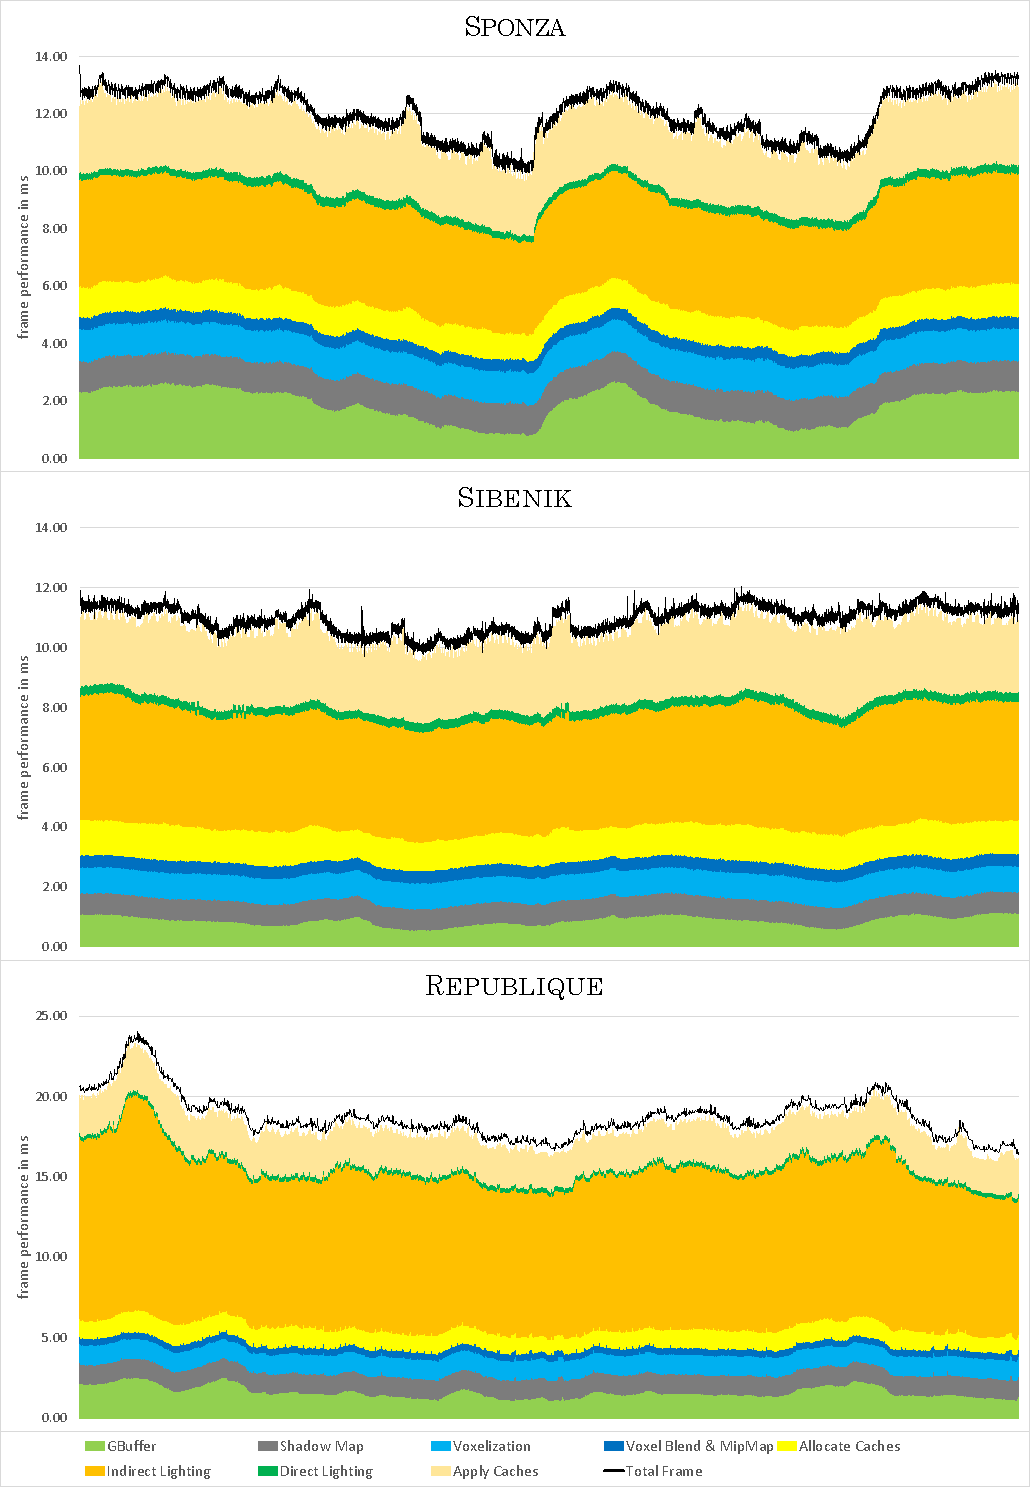
\includegraphics[width=\textwidth]{eva/breakdown/specoff.pdf}
\caption{Timing breakdown with a moving camera (for 30s) for indirect diffuse lighting. x-axis: frame index, y-axis: stacked duration.}
\label{fig:frameratebreakdown:specoff}
\end{figure}
\begin{figure}
\centering
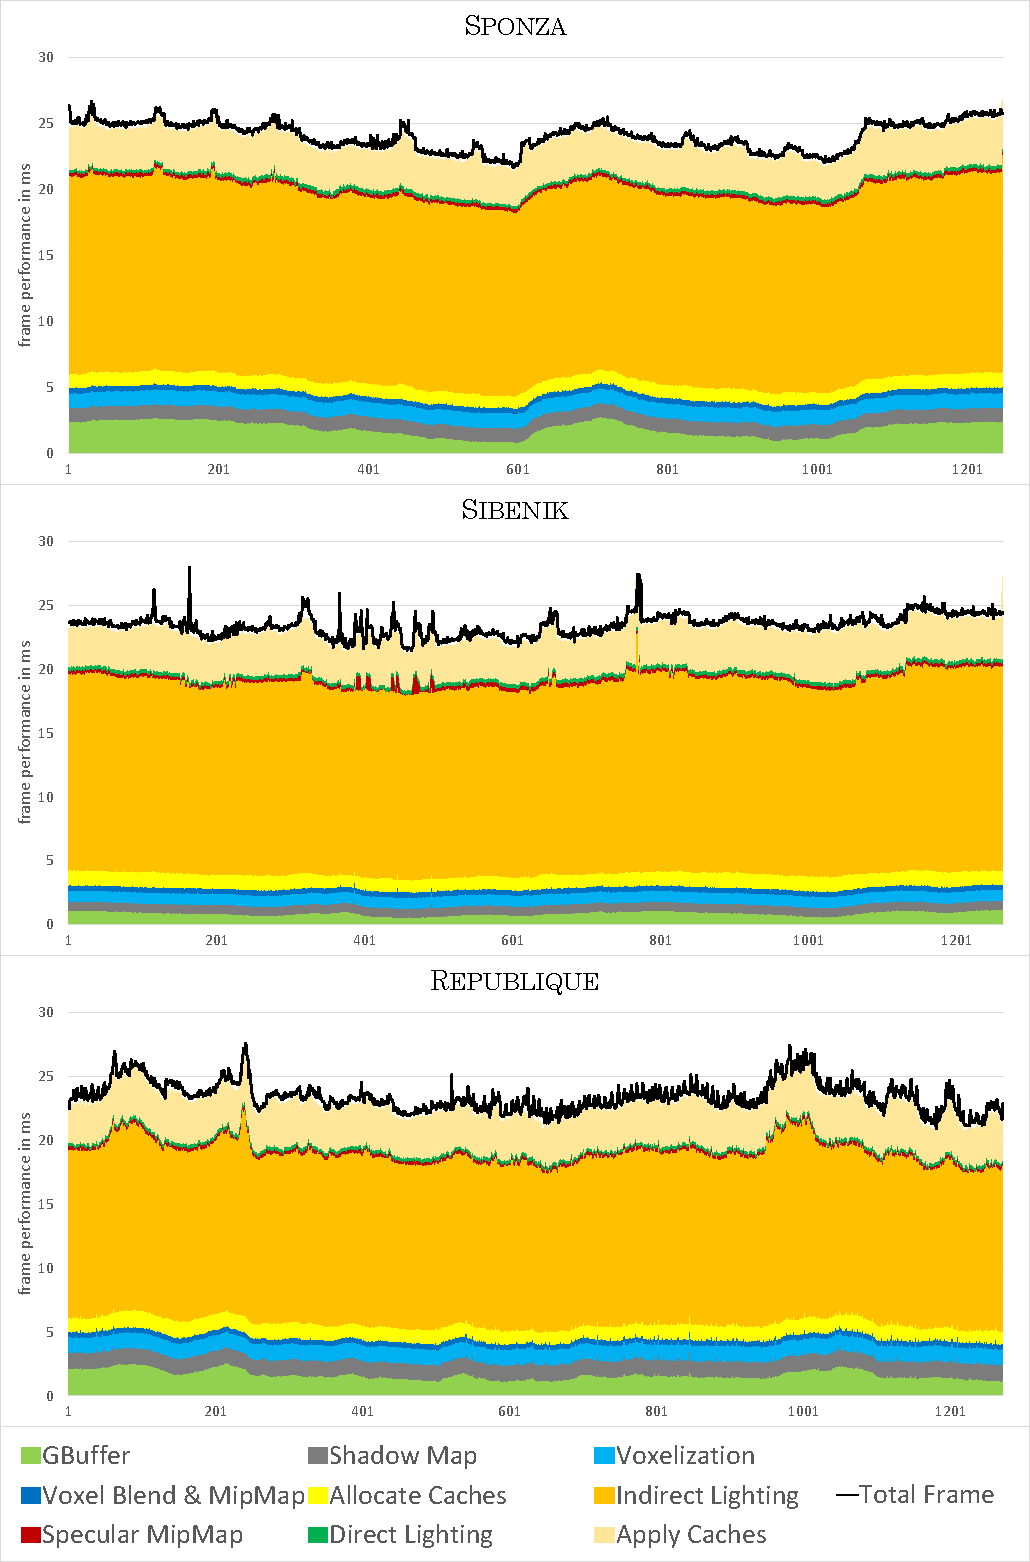
\includegraphics[width=\textwidth]{eva/breakdown/specon.pdf}
\caption{Timings with a moving camera  (for 30s) for indirect diffuse \& \emph{specular} lighting. x-axis: frame index, y-axis: stacked duration.}
\label{fig:frameratebreakdown:specon}
\end{figure}

First, we want to provide a general overview over how long the different steps of our rendering pipeline usually take.
For this, we measure all timings along 30 seconds camera flights through our test scenes using the default settings mentioned in \autoref{sec:eva:setup}.
These paths are shown by the accompanying videos.
The first set of graphs in \autoref{fig:frameratebreakdown:specoff} shows timings without and the second in \autoref{fig:frameratebreakdown:specon} with indirect specular reflections.
The stacked area plots are sorted in the order in which the respective passes are issued, starting with the G-buffer creation (light green) at the bottom and ending with the cache interpolation on top (beige).
The black line at the top of all plots shows the total duration for each recorded frame.
Note that there is a small white gap bellow this line which represents the duration of all overheads that were not measured explicitly like tonemapping, several uniform buffer updates and output to the backbuffer.

As can be seen easily, the indirect specular lighting increases the costs of the indirect lighting pass (dark yellow) considerably while the additional mipmapping of the specular environment map is very cheap.
Since the light does not move in these tests, the rendering of the reflective shadow map (dark grey) is constant over time.
The duration of the voxelization pass and its blending + mipmapping is constant as well since there are no changes in resolution or the geometrical complexity of the scene.
More surprisingly, there are also almost no changes over time in the cache allocation pass (bright yellow) even when the cache lighting pass (dark yellow) is significantly slower which hints a higher number of light caches.
Since the main influence to this and the other two cache related passes is the number of active caches we will investigate this further in the next section on cache count. 
The strong changes in the duration of the G-buffer creation pass (especially in \dataset{Sponza}) stems from varying overdraw depending on the current view orientation.

In general, the performance in the three scenes does not differ much.
Only the significantly more complex \dataset{Republique} scene performs a bit slower which is observable especially without indirect specular.

\subsection{Cache Count}
Retrieving the current cache count from the GPU is a very costly operation unless extensive multi-buffering is used to avoid stalls (i.e. keeping the count in a different buffer every frame to ensure that all reads are performed on an unused one).
Therefore, we measured the cache count over time separately and combined the results in the graphs seen in \autoref{fig:cachecountovertime}.

\begin{figure}
\centering
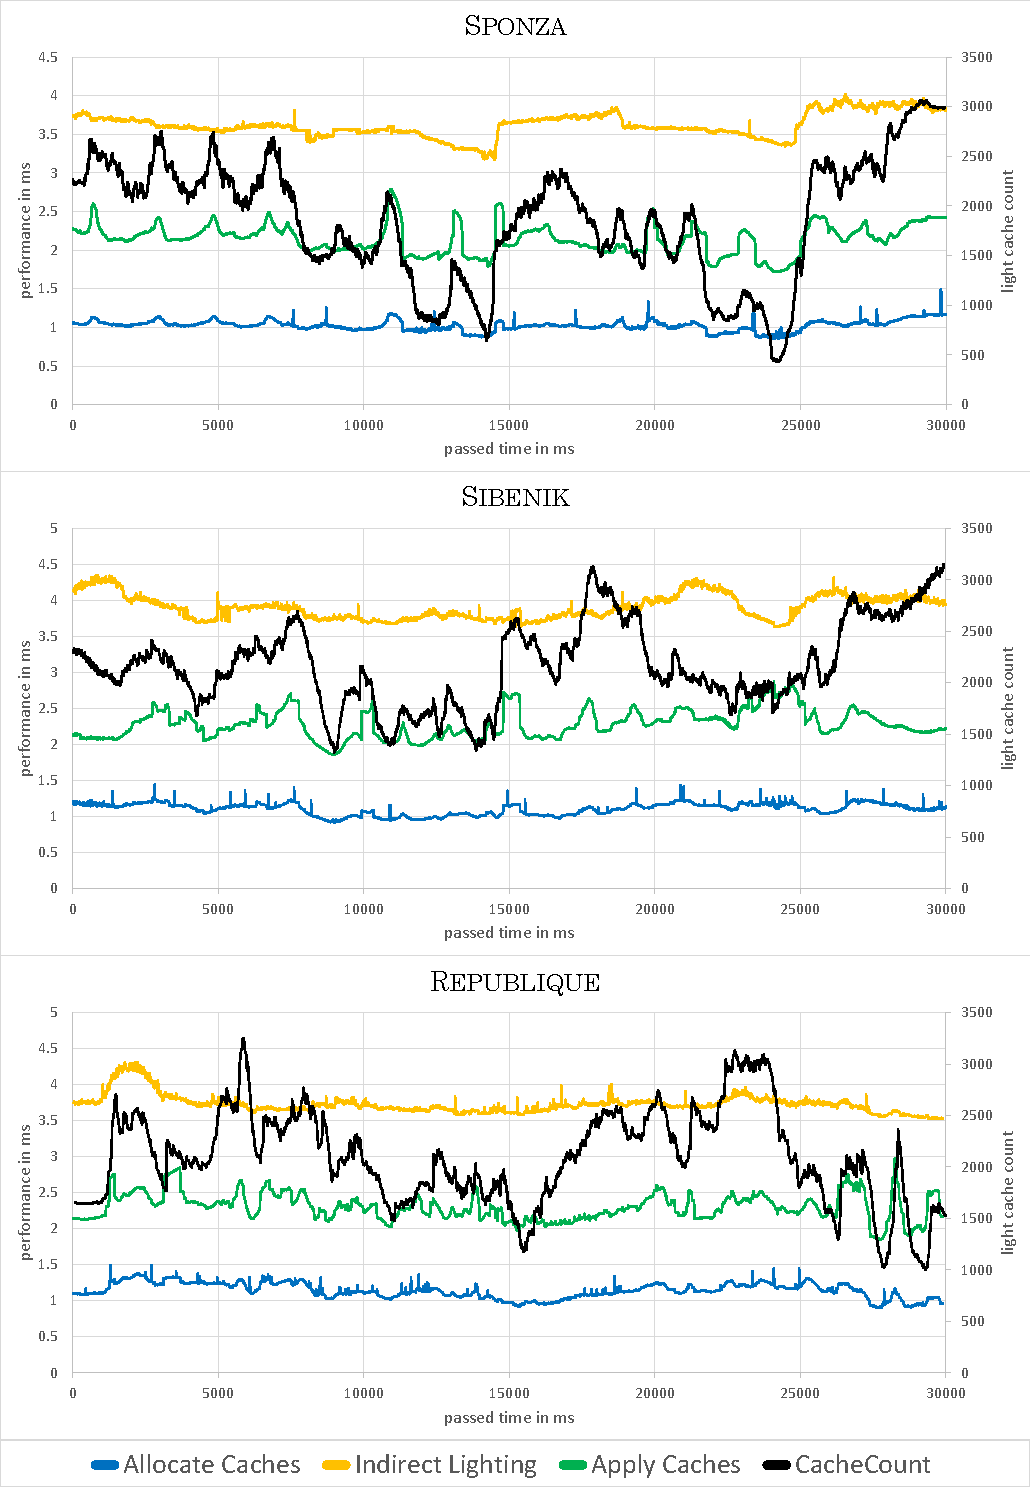
\includegraphics[width=\textwidth]{eva/cachecountovertime/combined.pdf}
\caption{Visualization of the influence of cache count (black) to all relevant passes over time (30s), using the same camera flights and settings as in \autoref{fig:frameratebreakdown:specoff}.}
\label{fig:cachecountovertime}
\end{figure}
Surprisingly, there seems to be only a slight correlation between the duration of the cache lighting pass and the number of caches.
The duration of the allocate pass is rather stable over time and only the apply cache pass shows a slight and very unsteady correlation to the cache count.
The steadiness of the cache allocation pass comes most likely from the fact that on average every thread group performs a single cache allocation attempt regardless of the cache count.
Weather an attempt is redundant or not might not be as important for the runtime.
The cache apply pass on the other hand has a strict control flow, i.e. it executes the same code insensitive to the number of caches.
This leaves only the changing number of cache misses as reasonable explanation for its behavior.
\\
\begin{figure}[h]
\centering
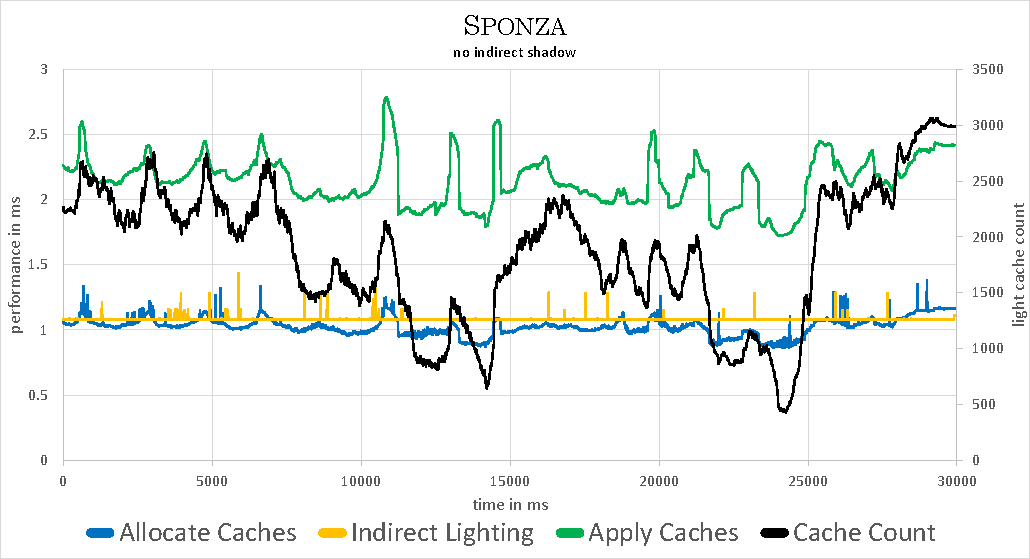
\includegraphics[width=\textwidth]{eva/cachecountovertime/sponza_noshadow.pdf}
\caption{Cache count (black) in comparison to indirect lighting passes with inactive indirect shadowing (camera path and other settings as in \autoref{fig:frameratebreakdown:specoff}).}
\label{fig:cachecountovertime:noshadow}
\end{figure}
\\
Clearly, the main bottleneck of the cache lighting pass in the preceding tests is not the raw number of caches to be lit, but another factor that changed along the tested camera paths.
To reduce the number of influences we ran the same experiment in the \dataset{Sponza} scene again with disabled indirect shadow.
\\
The results, seen in \autoref{fig:cachecountovertime:noshadow}, show an even more extreme picture:
Now the duration of the caching pass is almost completely constant, while correlations of the cache count and the performance of the other two parts are much better visible.
Naturally we suspected a bug in the implementation of the light caching pass that is expected to a have linear performance characteristic in respect to the number of active light caches.
However, more experiments with higher cache counts show that there is in fact such a linear correlation.
This time we chose a fixed view point in the \dataset{Sponza} scene, using the default non-specular settings and measure the performance (and cache count) for different CAV resolutions.
The results are plotted in \autoref{fig:cachecountdirect}.
\\
\begin{figure}[h]
\centering
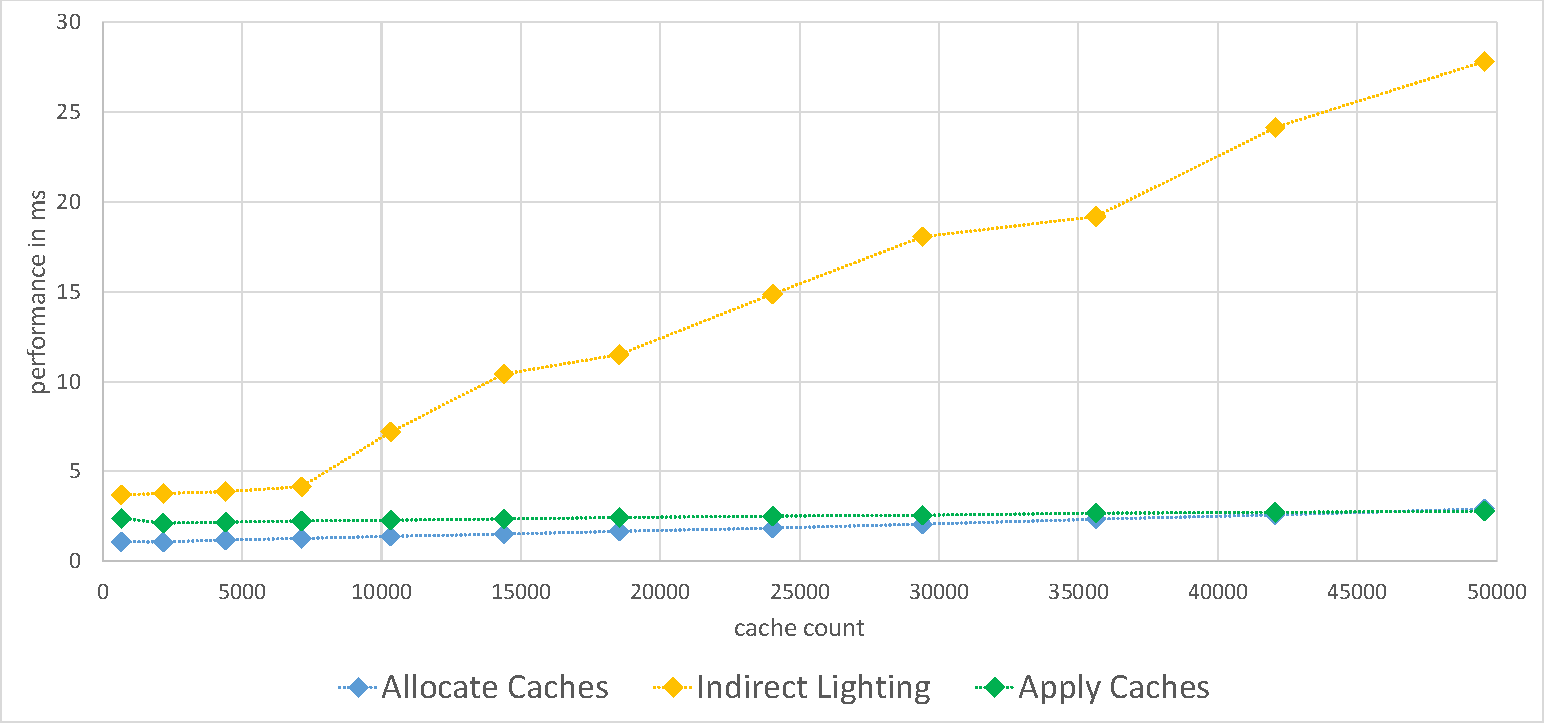
\includegraphics[width=\textwidth]{eva/cachecount.pdf}
\caption{Performance for different cache counts. Recorded in \dataset{Sponza} with varying CAV resolutions, starting with $16^3$, ending with $192^3$. Otherwise default settings without indirect specular. }
\label{fig:cachecountdirect}
\end{figure}
The implementation of the cache lighting pass uses 512 threads per group since it performed best on average with this count.
As the shared memory optimization (see \autoref{sec:impl:details:lighting}) enforces that all threads of a group remain active, this is also the lowest theoretical granularity to which the performance of this pass can react.
Obviously though, due to the characteristics of our graphics card (number of multiprocessors, minimum/maximum parallel thread groups in flight etc.), the measured granularity is much coarser, especially for a low number of thread groups.
More experiments with different thread group sizes would be necessary for a deeper insight into this matter.
\\
This experiment also shows that the allocate pass is more sensible to the cache count than the apply pass for large cache counts.

\subsection{SH Band Count} \label{sec:eva:shperf}
For diffuse lighting we use either two or three spherical harmonics bands.
Using more or a generic count of bands was considered too complex to implement for the large associated performance hit that is expected to bring only slight improvement in lighting.
In fact, already switching from two to three bands can result in a much costlier cache apply pass, as can be seen in \autoref{tab:shperf}.
\begin{table}[htbp]
  \centering
    \begin{tabular}{r|rr|rr|rr}
    \toprule
          & \multicolumn{2}{c|}{CAV $32^3$ (2177)} & \multicolumn{2}{c|}{CAV $64^3$ (7128)} & \multicolumn{2}{c}{CAV $128^4$ (24033)} \\
    \midrule
          & \small{Ind. Lighting} & Apply & Ind. Lighting & Apply & Ind. Lighting & Apply \\
    \midrule
    2 bands & 3.75  & 2.12  & 4.16  & 2.25  & 14.8  & 2.51 \\
    3 bands & 3.98  & 3.83  & 4.58  & 4.14  & 16.7  & 4.74 \\
    \bottomrule
    \end{tabular}
\caption{Performance of indirect lighting and cache apply passes in \si{\milli\second} for different numbers of spherical harmonics bands and CAV resolutions (resulting cache counts in parenthesis) in the \dataset{Sponza} scene. }
\label{tab:shperf}
\end{table}
The increased band count means higher register pressure and more arithmetic for the indirect lighting pass as well.
However, as the numbers show, the impact is here more limited.
Since the main bottleneck is the visibility calculation, a few more or less arithmetic instructions do not have a large influence.
Other passes are obviously not affected by the precision of our spherical harmonics representation.

\subsection{RSM Resolution}
\begin{table}[h]
  \centering
    \begin{tabular}{r|rrr}
    \toprule
    \multirow{2}{*}{RSM resolution} & \multicolumn{3}{c}{ shadow/specular}\\
     & off/off & on/off & on/on \\
    \midrule
    $16^2$    & 0.220 & 1.423 & 3.276 \\
    $32^2$    & 0.419 & 2.480 & 6.138 \\
    $64^2$    & 1.200 & 3.875 & 16.260 \\
    $128^2$   & 4.311 & 9.710 & 50.160 \\
    $256^2$   & 16.764 & 38.419 & 155.660 \\
    $512^2$   & 66.587 & 154.771 & 400.265 \\
    \bottomrule
    \end{tabular}
\caption{Performance of the cache lighting pass in \si{\milli\second} for different reflective shadow map resolutions in the \dataset{Republique} scene. All tests the used same number of shadow cones. }
\label{tab:RSMsizeperf}
\end{table}
The reflective shadow map resolution has a major impact on the duration of the indirect lighting pass which is practically always the slowest step in our rendering process.
\autoref{tab:RSMsizeperf} shows its influence on the performance in the \dataset{Republique} scene with a fixed view point that activates 3045 caches.
Increasing the size of the reflective shadow map also increases the number of shadow cones per cache.
Since we are only interested in the effects of the RSM resolution we canceled that factor out by increasing the shadow LODs so that the number of cones stays at 256.
\\
Resolutions beyond $128^2$ are practically not usable from a real-time performance standpoint, regardless of weather indirect shadows and specular effects are activated or not.

\subsection{Indirect Shadow}
Comparing the statistics on cache count influence with (see \autoref{fig:cachecountovertime}) and without shadowing (see \autoref{fig:cachecountovertime:noshadow}) we can already deduce that indirect shadowing has a rather high performance impact depending on the visible scene portion which determines the average length of the shadow cones.
More important though is the shadow LOD since it determines together with the RSM resolution how many shadow cones are needed for each cache.
\\
\begin{table}[h]
  \centering
    \begin{tabular}{c|rrrrr}
    \toprule
    \diagbox[width=8.5em]{\small{shadow}\scriptsize{ LOD}}{\small{RSM res.}} \,\,    & $16^2$ & $32^2$ & $64^2$ & $128^2$ & $256^2$ \\
    \midrule
    0     & 2.16  & 8.89  & 36.91 & 150.09 & 538.45 \\
    1     & 0.62  & 2.48  & 10.06 & 44.21 & 231.43 \\
    2     & 0.33  & 0.97  & 3.87  & 15.73 & 67.37 \\
    3     & 0.29  & 0.71  & 2.45  & 9.70  & 39.12 \\
    4     & 0.29  & 0.67  & 2.19  & 8.35  & 33.29 \\
    5     &       & 0.66  & 2.15  & 8.11  & 32.00 \\
    6     &       &       & 2.15  & 8.08  & 31.79 \\
    7     &       &       &       & 8.08  & 31.81 \\
    8     &       &       &       &       & 31.79 \\
    \bottomrule
    \end{tabular}
\caption{Performance of the cache lighting pass in \si{\milli\second} for different shadow LODs and RSM resolutions in the \dataset{Republique} scene.}
\label{tab:shadowlod}
\end{table}
\\
\autoref{tab:shadowlod} shows measurements of the duration of the cache lighting pass depending on shadow LOD and reflective shadow map resolution.
The last entry in each column was rendered with a single large shadow cone. 
Each entry above used a quadrupled number of shadow cones.

Another important parameter is the resolution of the voxel volume.
For simplicity, the application only supports cubic volumes that are aligned to the entire scene.
This results in rather poor voxel space usage as all our scenes have a larger extent on a single dominant axis.
\\
\begin{table}[h]
  \centering
    \begin{tabular}{r|rrrrr}
    \toprule
    \diagbox[width=8.5em]{\small{shadow}\scriptsize{ LOD}}{\small{Voxel res.}} \,\, & $32^3$ & $64^3$ & $128^3$ & $256^3$ & $512^3$ \\
    \midrule
    0     & 22.22 & 29.61 & 36.91 & 112.07 & 301.33 \\
    1     & 6.89  & 8.60  & 10.06 & 24.23 & 68.54 \\
    2     & 3.26  & 3.56  & 3.87  & 6.03  & 16.69 \\
    3     & 2.34  & 2.41  & 2.45  & 2.64  & 3.29 \\
    4     & 2.18  & 2.19  & 2.19  & 2.21  & 2.24 \\
    5     & 2.15  & 2.15  & 2.15  & 2.16  & 2.16 \\
    6     & 2.15  & 2.15  & 2.15  & 2.15  & 2.15 \\
    \bottomrule
    \end{tabular}
\caption{Performance of the cache lighting pass in \si{\milli\second} for different shadow LODs and voxel volume resolutions in the \dataset{Republique} scene. RSM resolution was fixed to $64^2$.}
\label{tab:shadowvoxelres}
\end{table}
\\
\autoref{tab:shadowvoxelres} shows how the resolution of the voxel volume influences the duration of the cache lighting pass.
For unrealistic high shadow LODs there is almost no difference in performance for different voxel resolutions.
This can easily be explained by the fact that a high shadow LOD results in large cones that take only few samples in high order mip-levels, thus using a low resolution version of the voxelization anyways.
\\
We deliberately did not include measurements on how long the voxelization takes, as this was discussed in the works from which our voxelization-implementation is derived.

\subsection{Indirect Specular} \label{sec:eva:specperf}
\begin{table}[h]


\definecolor{bad0}{RGB}{248,105,107}
\definecolor{bad1}{RGB}{248,113,108}
\definecolor{bad2}{RGB}{250,149,115}
\definecolor{bad3}{RGB}{249,134,112}
\definecolor{bad4}{RGB}{249,134,112}
\definecolor{bad5}{RGB}{251,178,121}
\definecolor{neutral0}{RGB}{254,226,130}
\definecolor{neutral1}{RGB}{251,234,132}
\definecolor{neutral2}{RGB}{225,227,131}
\definecolor{neutral3}{RGB}{253,235,132}
\definecolor{neutral4}{RGB}{238,230,131}
\definecolor{good0}{RGB}{118,196,125}
\definecolor{good1}{RGB}{99,190,123}
\begin{subtable}{\textwidth}
	\centering
	\begin{tabular}{c|rrrrr}
	\toprule
	 \diagbox[width=10em]{\small{spec. map res.}}{\small{RSM res.}} \,\, & $16^2$    & $32^2$    & $64^2$    & $128^2$   & $256^2$ \\
	\midrule
	$4^2$     & \cellcolor{neutral3} 1.04  & \cellcolor{bad2} 3.05  & \cellcolor{bad1} 11.14 & \cellcolor{bad0} 43.20 & \cellcolor{bad0} 170.39 \\
	$8^2$     & \cellcolor{neutral4} 1.16  & \cellcolor{bad5} 3.48  & \cellcolor{bad4} 12.83 & \cellcolor{bad3} 49.67 & \cellcolor{bad3} 195.66 \\
	$16^2$    & \cellcolor{good0} 1.30  & \cellcolor{neutral2} 3.62  & \cellcolor{neutral1} 12.95 & \cellcolor{neutral0} 49.86 & \cellcolor{neutral0} 195.87 \\
	$32^2$    & \cellcolor{good1} 1.72  & \cellcolor{good1} 4.07  & \cellcolor{good0} 13.33 & \cellcolor{good0} 49.96 & \cellcolor{good0} 195.24 \\
	$64^2$    & \cellcolor{good1} 3.42  & \cellcolor{good1} 5.78  & \cellcolor{good1} 15.06 & \cellcolor{good1} 51.76 & \cellcolor{good1} 196.83 \\
	\bottomrule
	\end{tabular}
	\caption{Direct write.\vspace{0.5cm}}
\end{subtable}

\definecolor{good0}{RGB}{99,190,123}
\definecolor{good1}{RGB}{143,203,126}
\definecolor{good2}{RGB}{118,196,125}
\definecolor{good3}{RGB}{176,213,128}
\definecolor{neutral0}{RGB}{254,234,131}
\definecolor{neutral1}{RGB}{254,230,131}
\definecolor{neutral2}{RGB}{242,239,132}
\definecolor{bad0}{RGB}{251,167,119}
\definecolor{bad1}{RGB}{250,148,115}
\definecolor{bad2}{RGB}{248,105,107}
\definecolor{bad3}{RGB}{251,177,120}
\definecolor{badextra}{RGB}{248,105,107}
\begin{subtable}{\textwidth}
	\centering
	\begin{tabular}{c|rrrrr}
	\toprule
	 \diagbox[width=10em]{\small{spec. map res.}}{\small{RSM res.}} \,\, & $16^2$    & $32^2$    & $64^2$    & $128^2$   & $256^2$ \\
	\midrule
	$4^2$     & \cellcolor{neutral0} 0.74  & \cellcolor{good1} 1.74  & \cellcolor{good0} 5.89  & \cellcolor{good0} 22.50 & \cellcolor{good0} 88.66 \\
	$8^2$     & \cellcolor{neutral0} 0.90  & \cellcolor{good3} 2.12  & \cellcolor{good2} 7.09  & \cellcolor{good2} 26.92 & \cellcolor{good2} 105.93 \\
	$16^2$    & \cellcolor{bad0} 3.75  & \cellcolor{neutral1} 3.05  & \cellcolor{neutral0} 9.32  & \cellcolor{neutral2} 34.43 & \cellcolor{neutral2} 134.22 \\
	$32^2$    & \cellcolor{bad2} 8.48  & \cellcolor{bad1} 14.34 & \cellcolor{bad0} 37.82 & \cellcolor{bad3} 131.00 & \cellcolor{bad3} 501.43 \\
	$64^2$    & \multicolumn{5}{c}{\cellcolor{badextra} \emph{application crash}} \\
	\bottomrule
	\end{tabular}
	\caption{\centering Register cached write. }
\end{subtable}
\caption{Performance of the cache lighting pass in \si{\milli\second} for different specular environment and RSM resolutions in the \dataset{Sponza} scene. The colors indicate where direct writing to the map or caching in the shader's registers is better.}
\label{tab:specularperf}
\end{table}

So far we have ignored the effect of indirect specular lighting, except in the breakdown overview in \autoref{fig:frameratebreakdown:specon}.
Indirect specular lighting in general has a severe impact on the performance.
\\
As noted in \autoref{sec:impl:details:specular} there are two ways to handle writes to the specular environment map:
Either by writing directly into it or by caching the map in the shader's registers.
\autoref{tab:specularperf} shows timings of the indirect lighting pass in the \dataset{Sponza} scene with varying RSM and specular environment map resolutions for both direct and cached write.
The RSM resolution determines how often writes to the specular environment map occur.
Using cached writes, specular environment maps with a resolution of $8^2$ and lower are clearly faster on our machine.
For $16^2$ it depends and $64^2$ lead to a crash on our machine since the driver was not able to compile the shader (which indicates a driver bug since there was no controlled error output).
\\
For direct writes, the performance is very stable independently of the specular environment map resolution.
However, this parameter can also raise memory requirements drastically (see also \autoref{sec:eva:memory}).

\subsection{Resolution Dependence}
Finally, we want to test the effect of the screen resolution on our global illumination algorithm.
Both the cache allocation and interpolation (= apply) passes are executed for every screen pixel.
As expected, our tests in \autoref{fig:resolutionperf} show an almost linear correlation to the number of screen pixels.
The duration of the allocate pass increases especially slowly with the resolution compared with the allocate and apply passes.
For this test we used the \dataset{Sibenik} scene and increased the CAV resolution to $64^3$ for a higher cache density.
%Measurement inaccuracies can arise from the different aspect ratios which lead to slightly varying cache counts for different resolution configurations.
\begin{figure}[h!]
\centering
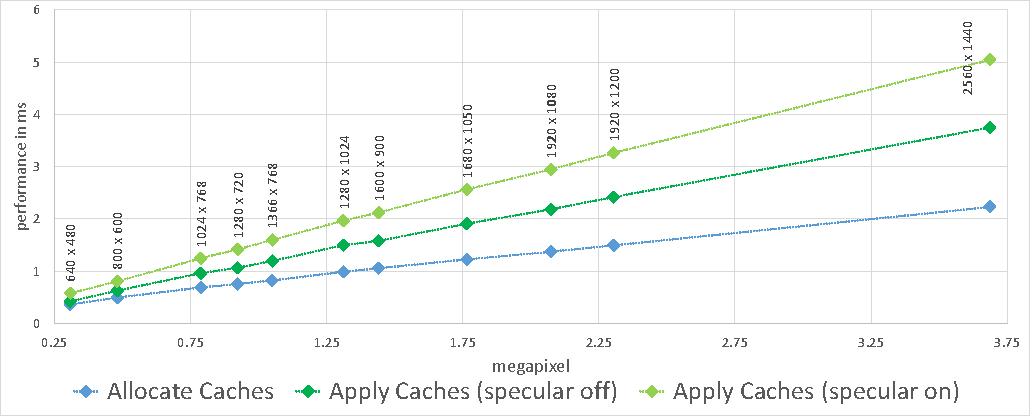
\includegraphics[width=\textwidth]{eva/screen_resolution.pdf}
\caption{Performance of cache allocation and interpolation in \si{\milli\second} at different screen resolutions in \dataset{Sibenik} scene. Used CAV with $64^3$, resulting in about 7300 caches.}
\label{fig:resolutionperf}
\end{figure}

\newpage
\section{Quality}
While the previous section examined the effect of several parameters on how well the approach performs in terms of computation time, this section will try to evaluate its general visual quality.
%Unlike before, we will do this in a more feature oriented fashion instead of observing the effect of single configuration tweaks.

\subsection{Sources of Error} \label{sec:eva:errorsources}
There are several sources of error in regard to the ground-truth that is defined by the rendering equation.
As the approach does not claim to be able to compute several phenomenon at all, we limit these observation to the officially supported types of light-paths.
In addition to both specular and diffuse direct lighting, our approach is able to compute specular and diffuse lighting after a diffuse light bounce.
Like in the original reflective shadow mapping, our approach is not able to handle indirect specular light bounces which are necessary to compute caustics.

The reflective shadow map itself is the first source of error.
Problems arise from its limited resolution that determines how well the scene is sampled.
Low RSM lead to flickering during movement and irregular lighting, even with the bias compensation techniques which were discussed in \autoref{sec:fig:rsmbias}.
Also, small features may be missed entirely which leads to either to low or to high brightness in different areas.
Our approach to use down-sampled high resolution RSMs reduces flickering but creates virtual lights at inplausible in-between positions (as already mentioned in \autoref{sec:impl:rsmprep}).
\\
The discretized placement of light caches and their later interpolation has a similar effect on the overall accuracy, however in a more temporally stable fashion.
It assumes that there are no features of interest in-between two caches and that the transition can be expressed by simple linear interpolation.
\\
This is especially hazardous in combination with the RSM visibility approximation which is performed by cone-casts in a pre-filtered volume:
The higher the distance between the caches, the more likely is it that a cone starts within a solid object even when using a cache resolution dependent offset.
Voxel cone-casts assume that sampling the density information in arbitrary volume mipmap-levels expresses an isotropic visibility function for any cone going through this sample.
This estimate is more incorrect the more complex the geometry is which was combined into a single opacity value, i.e. it gets worse for higher mip-levels and lower resolutions.
Additionally, as we do not perform solid voxelization, blockers vanish in high mipmap-levels especially for a high starting resolution.
Larger cone angles produce higher errors as they perform samples more often in high mipmap-levels, while tight cones ray-march through (relatively) high-detailed volumes.
Testing multiple VALs at once with a single cone (shadow LOD) is based on the assumption that the visibility between arbitrary VALs does not vary much, which is obviously wrong for many cases.
\\
The two ways in which lighting information is saved have each their own accuracy issues.
Since our SH representation (for diffuse lighting) uses only very few bands, it can catch radiance only at very low frequencies.
Using higher SH basis would improve this but leads inevitably to stronger ringing artifacts.
While high frequencies are usually not necessary to estimate the irradiance, the representation is not entirely accurate.
The specular lighting on the other hand is limited by the per-cache specular environement map resolution that determines practically how large the maximal supported Blinn-Phong exponent is.
Saving only a hemisphere does not introduce any new errors but the hemispherical projection creates some distortion - to filter samples on this map is not identical with filtering on the hemisphere.
More importantly, the isotropic filtering process via mipmaps is flawed, as samples on higher mipmap-levels do not represent correct integrals over the anisotropic Blinn-Phong lobes.
However, in practice the largest error originates from the assumption that a single VAL does only affect a single pixel in the specular environment map.
This is more inaccurate with \emph{larger} specular environment map and lower RSM resolutions.
Note that all specular reflections can only show directly lit geometry due to the path length restrictions.

%\begin{easylist}
%# RSM
%## infinte size -> no error
%## single diffuse bounce
%# Cache discretization
%## infinite density -> every pixel lit individually
%# Shadow
%## bias
%## res
%# SH
%# SpecEnv
%\end{easylist}


%\subsection{Artifacts}
%regular placement of caches, jaggies,
%shadow jaggies,
%/interpolation issues
%
%shadow flickering?

\subsection{Groundtruth Comparision}
\begin{figure}[h]
\centering
\begin{subfigure}[b]{0.7\textwidth}
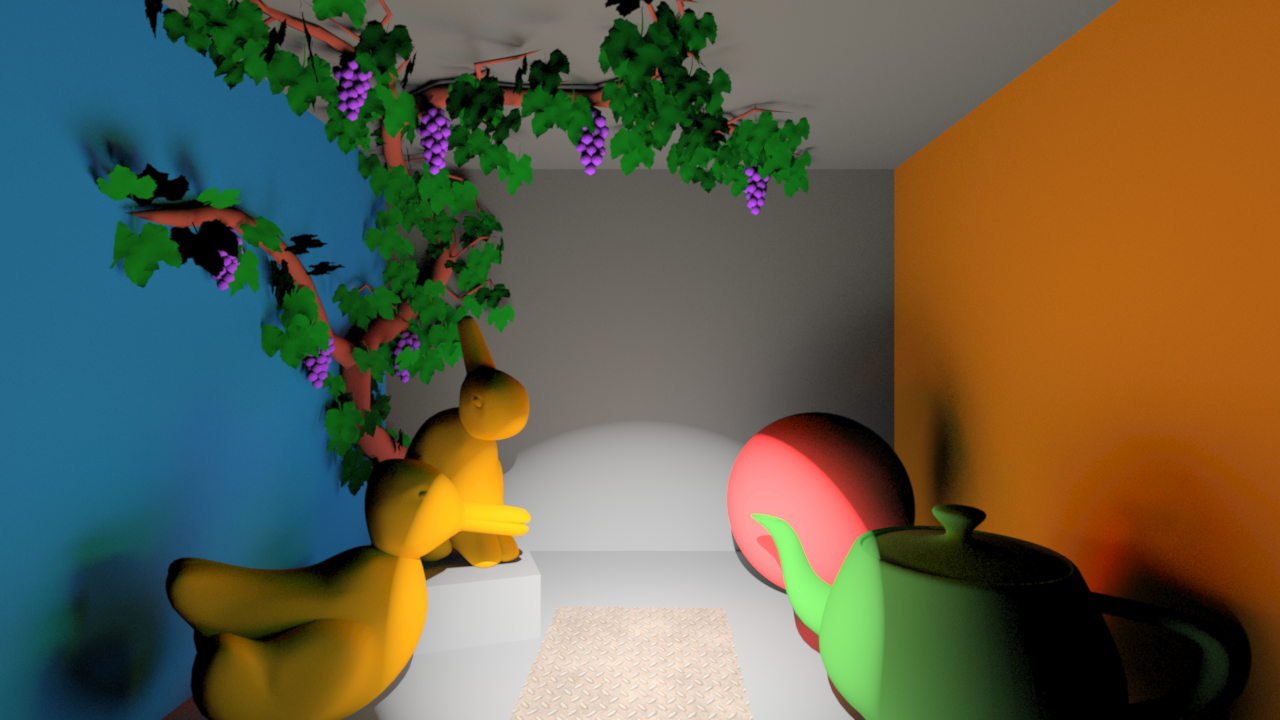
\includegraphics[width=\textwidth]{eva/groundtruthcomp/pathtracer}
\caption{Mitsuba \cite{bib:mitsuba} path-tracer, 2k samples per pixel ($\sim\SI{15}{\minute}$)}
\end{subfigure}
\\
\begin{subfigure}[b]{0.7\textwidth}
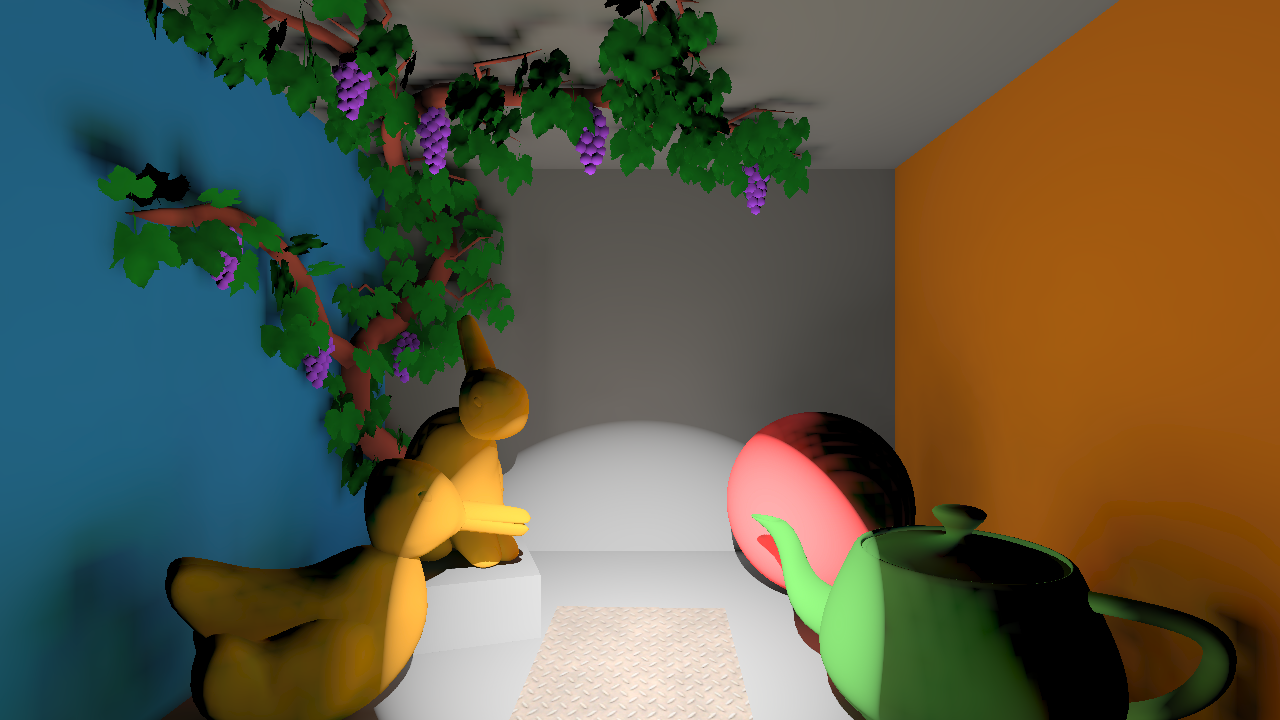
\includegraphics[width=\textwidth]{eva/groundtruthcomp/realtime}
\caption{Rendered with Dynamic Radiance Volumes ($\sim\SI{25}{\milli\second}$)}
\end{subfigure}
\caption{Comparison of a (diffuse only) scene rendered with the Mitsuba \cite{bib:mitsuba} path-tracer and with our realtime solution.}
\label{fig:groundtruthcomparision}
\end{figure}

\autoref{fig:groundtruthcomparision} shows renderings of a simple diffuse-only scene computed with Mitsuba's pathtracer \cite{bib:mitsuba} (top) and our technique (bottom).
Please note that we were not able to include such groundtruth images for the other scenes since it is rather difficult to share complex model and material setups in such way that fundamentally different renderers interpret them equally.
We chose a single address volume with a resolution of $128^3$, other than that we used the default settings without specular lighting since we were not able to replicate our BRDF setup in the path-tracer.
Using this rather high cache frequency, our approach is able to depict most shadowing details, however fails to compute them accurately.
The shadows are generally too bright and - not easily visible due to the tonemapping - tend to darken wide regions that should not be shadowed at all.
The brightening originates primarily from the thin voxelization which yields too low blocking values in higher voxel volume mipmaps levels.
The simple low frequent lighting in this scene though is no problem for our approach in general.
%Generally speaking, our technique is not able to reproduce high frequency changes in indirect lighting due to the rather sparse distribution of caches.
The jagged shadow border on the red ball originates from the regular cache distribution.
While it is rarely visible on textured surfaces, it is also very hard to avoid.

\subsection{SH Band Comparision} \label{sec:eva:shquality}
\begin{figure}[h]
\centering
\begin{subfigure}[b]{0.9\textwidth}
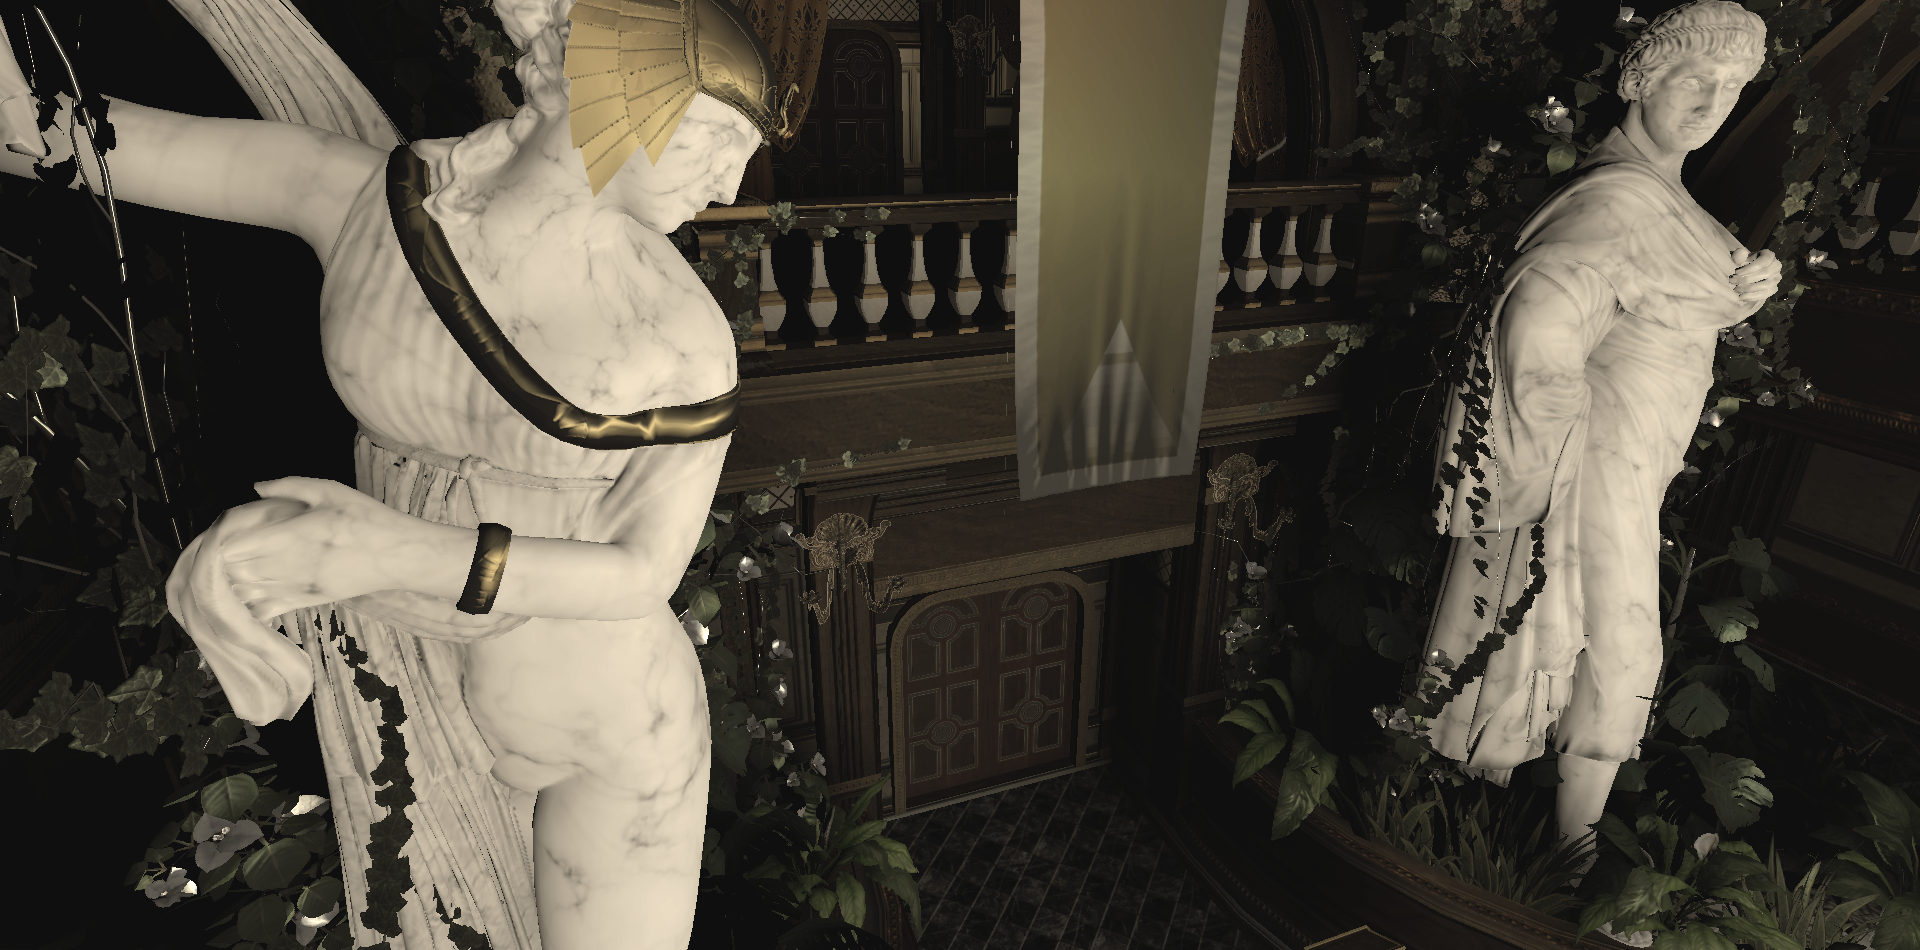
\includegraphics[width=\textwidth]{eva/sh/sh01}
\caption{2 SH bands.}
\end{subfigure}
\\
\begin{subfigure}[b]{0.9\textwidth}
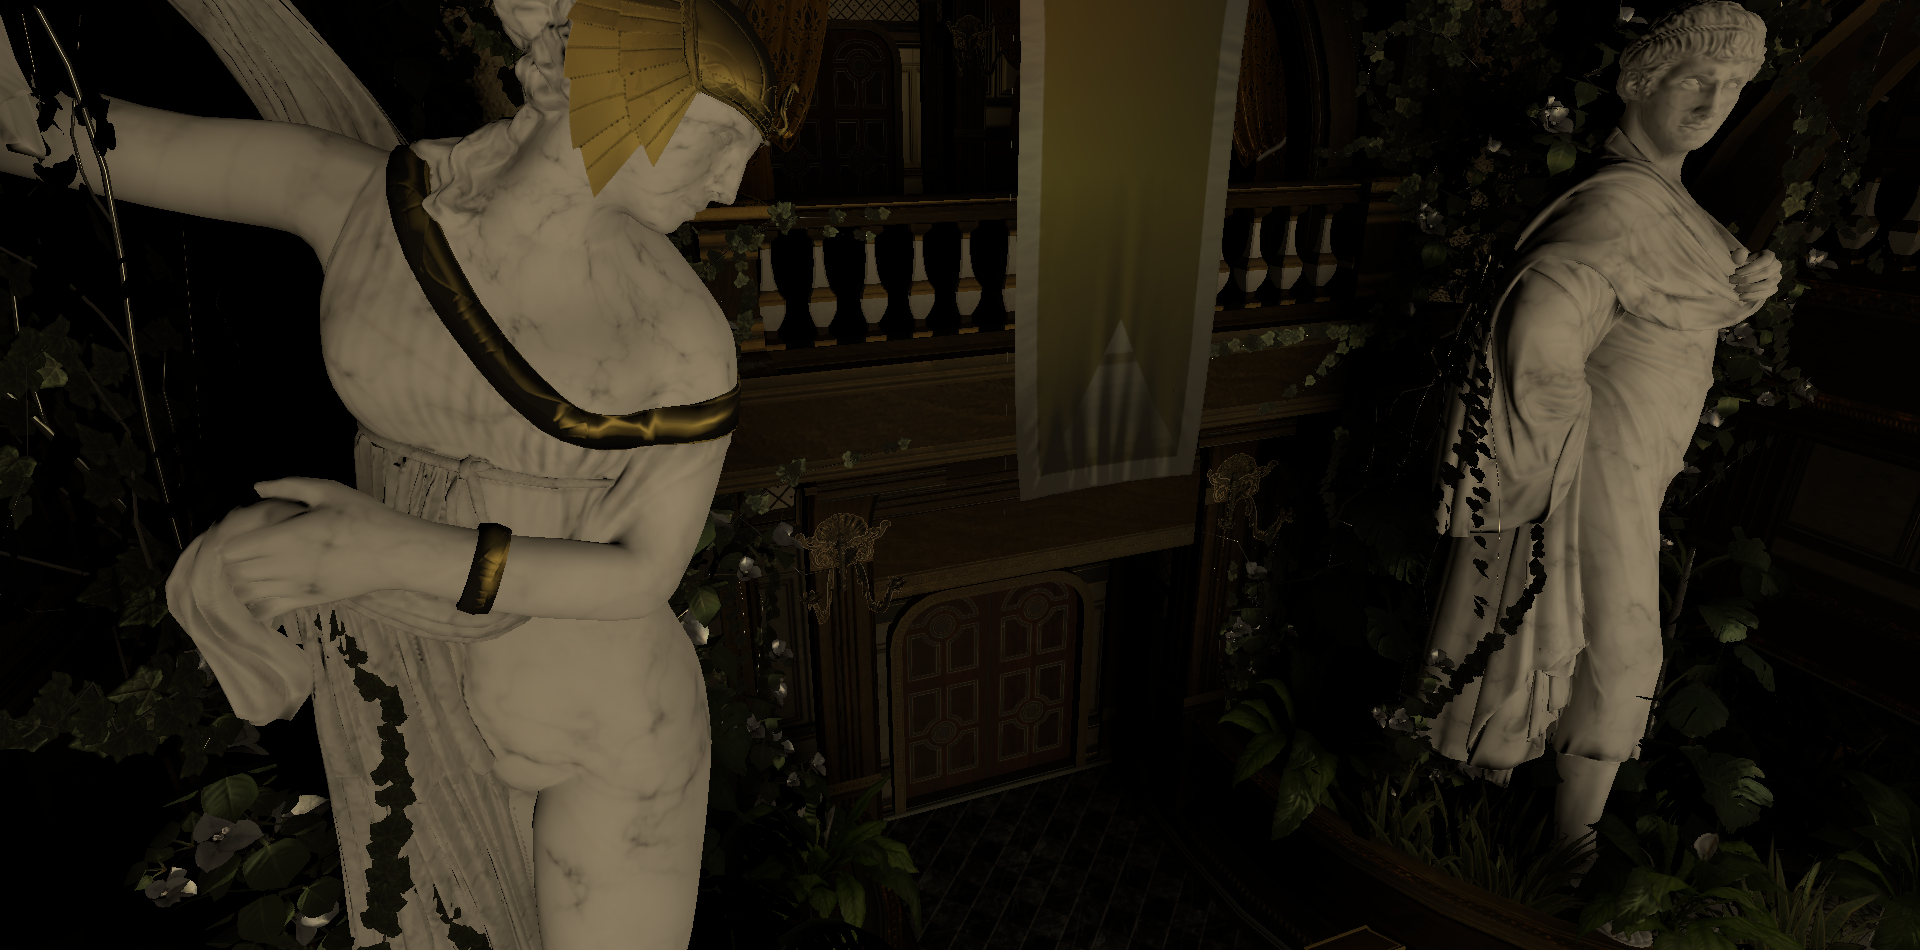
\includegraphics[width=\textwidth]{eva/sh/sh012}
\caption{3 SH bands.}
\end{subfigure}
\caption{Different spherical harmonics bases for diffuse lighting in the \dataset{Republique} scene.}
\label{fig:shcomparision}
\end{figure}
The quality difference between two or three spherical harmonics bands for diffuse lighting is often not very high.
\autoref{fig:shcomparision} shows an example with both negligible and rather good visible differences.
While the shading at the left statue changes only slightly, the right statue is more contrasted with three SH bands.
Generally, the setting with more SH bands displays crisper transitions between dark and bright zones but does not necessarily lead to more variations.
For example, the strongly normal-mapped flag in the middle of the scene barely changed.
For two or three SH bands we found almost no ringing artifacts in our test cases.

\subsection{Indirect Shadow}
\autoref{fig:shadowcomparision:resolutions} shows indirect shadow for different CAV and voxel resolutions.
In \autoref{fig:shadowcomparision:resolutions:cavdensities} the corresponding cache-density is visualized.
For a lower cache density there are sometimes jaggies visible at a shadows border.
Finer details get lost and Peter Panning is more likely to occur.
Using multiple cascades, the more distant cascades may have too few caches to represent the shadow at all, as can be seen in the corridor in the upper right of the images.
Higher voxel resolution has not only advantages:
While the shadow borders are more accurate (especially for high CAV resolutions), it is also disproportional brighter and tends to miss distant thin features since the volume is less dense in its higher mipmap-levels.
To avoid these issues, solid voxelization would be necessary.
\\
Similar behavior can be observed for the shadow LOD, see \autoref{fig:shadowcomparision:lod}.
With raising shadow LOD, the shadow gets brighter and thin features are more likely lost.
Besides, these images also feature the ability to produce "colored shadows" which are an implicit consequence of our technique.
%
\begin{figure}
\centering
\begin{subfigure}[b]{\halfpageimage}
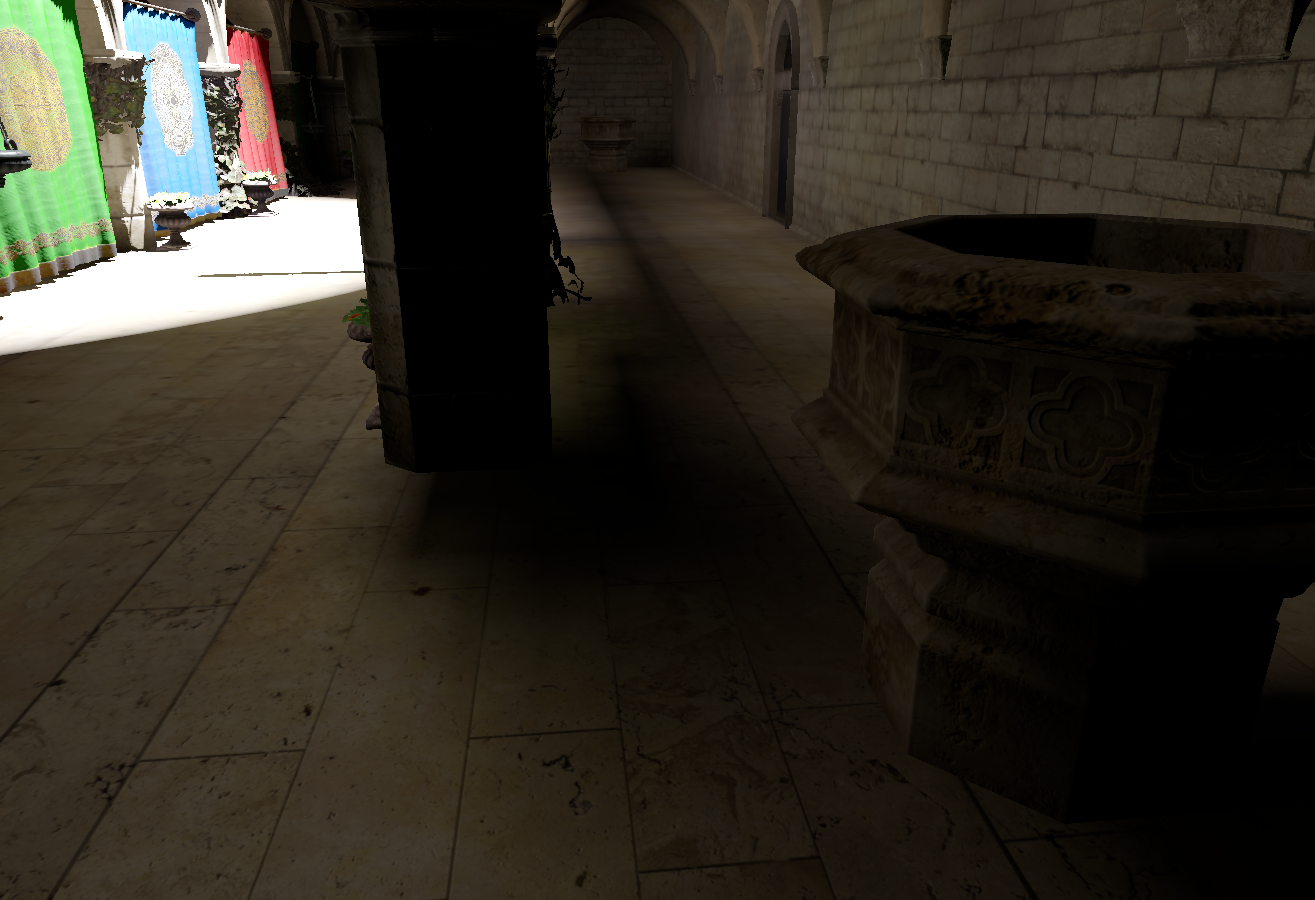
\includegraphics[width=\textwidth]{eva/shadow/vox128_cav32}
\caption{Voxelization: $128^3$ CAV: $4\times32^2$}
\end{subfigure}
\begin{subfigure}[b]{\halfpageimage}
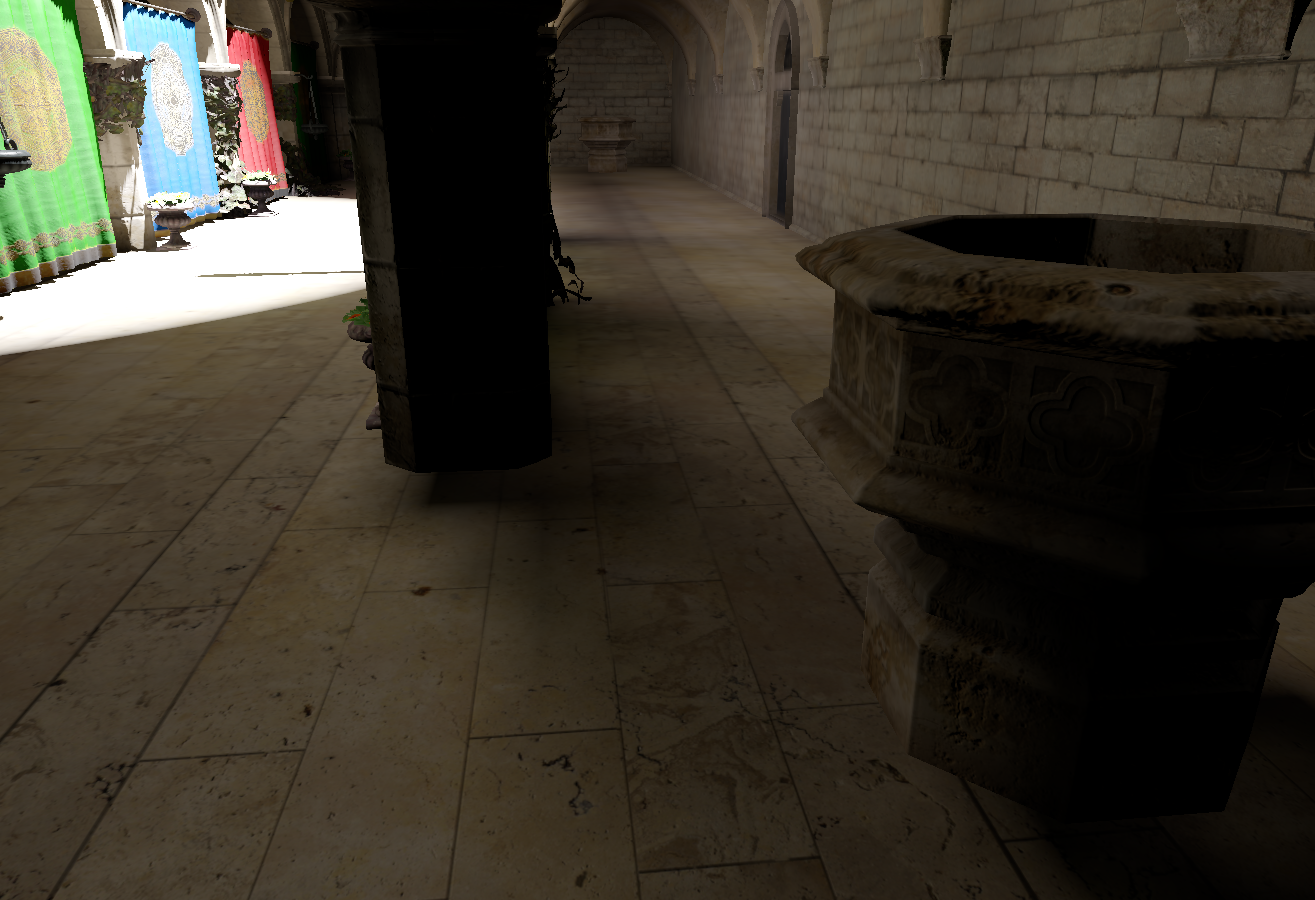
\includegraphics[width=\textwidth]{eva/shadow/vox256_cav32}
\caption{Voxelization: $256^3$ CAV: $4\times32^2$}
\end{subfigure}
\\
\begin{subfigure}[b]{\halfpageimage}
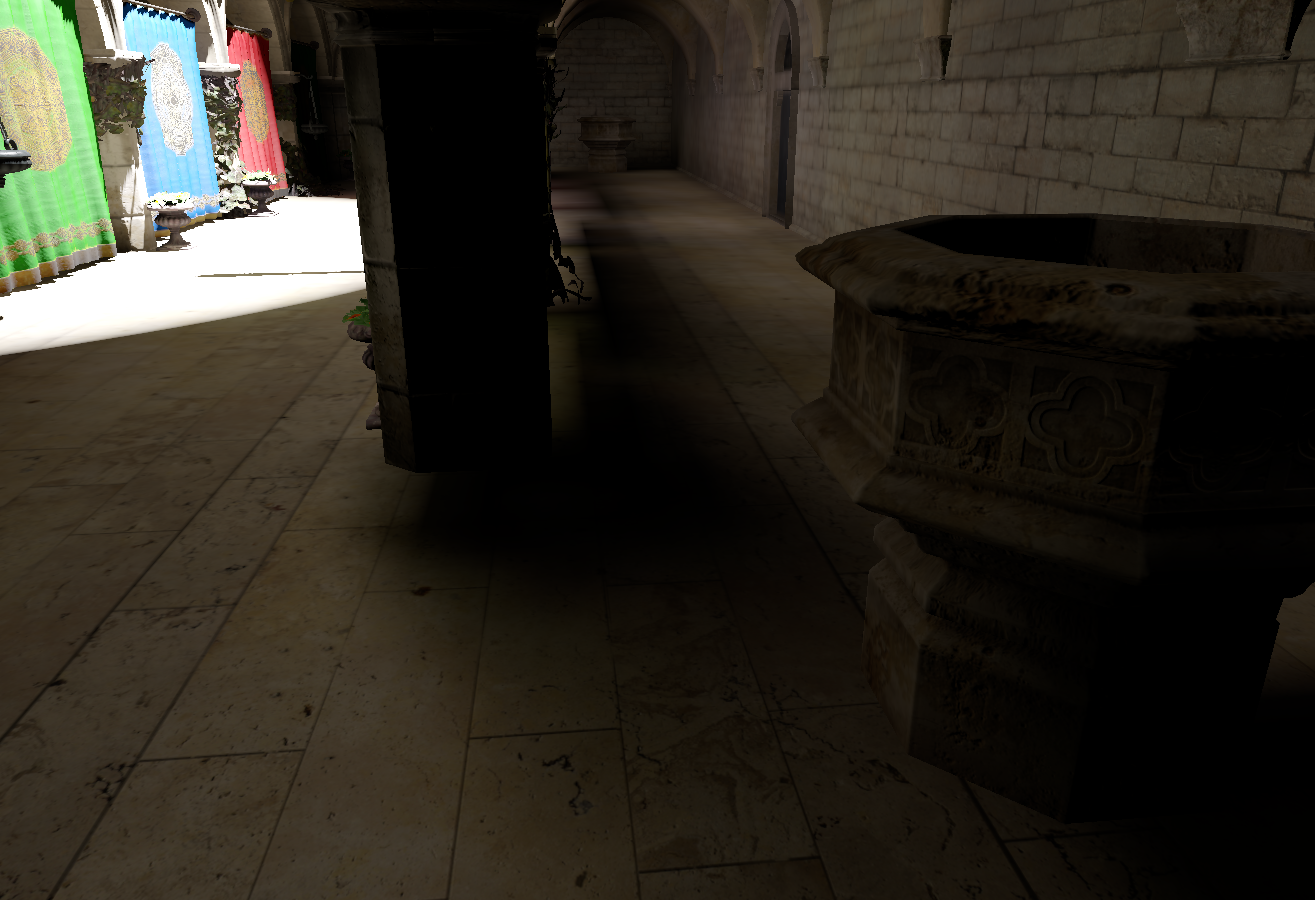
\includegraphics[width=\textwidth]{eva/shadow/vox128_cav64}
\caption{Voxelization: $128^3$ CAV: $4\times64^2$}
\end{subfigure}
\begin{subfigure}[b]{\halfpageimage}
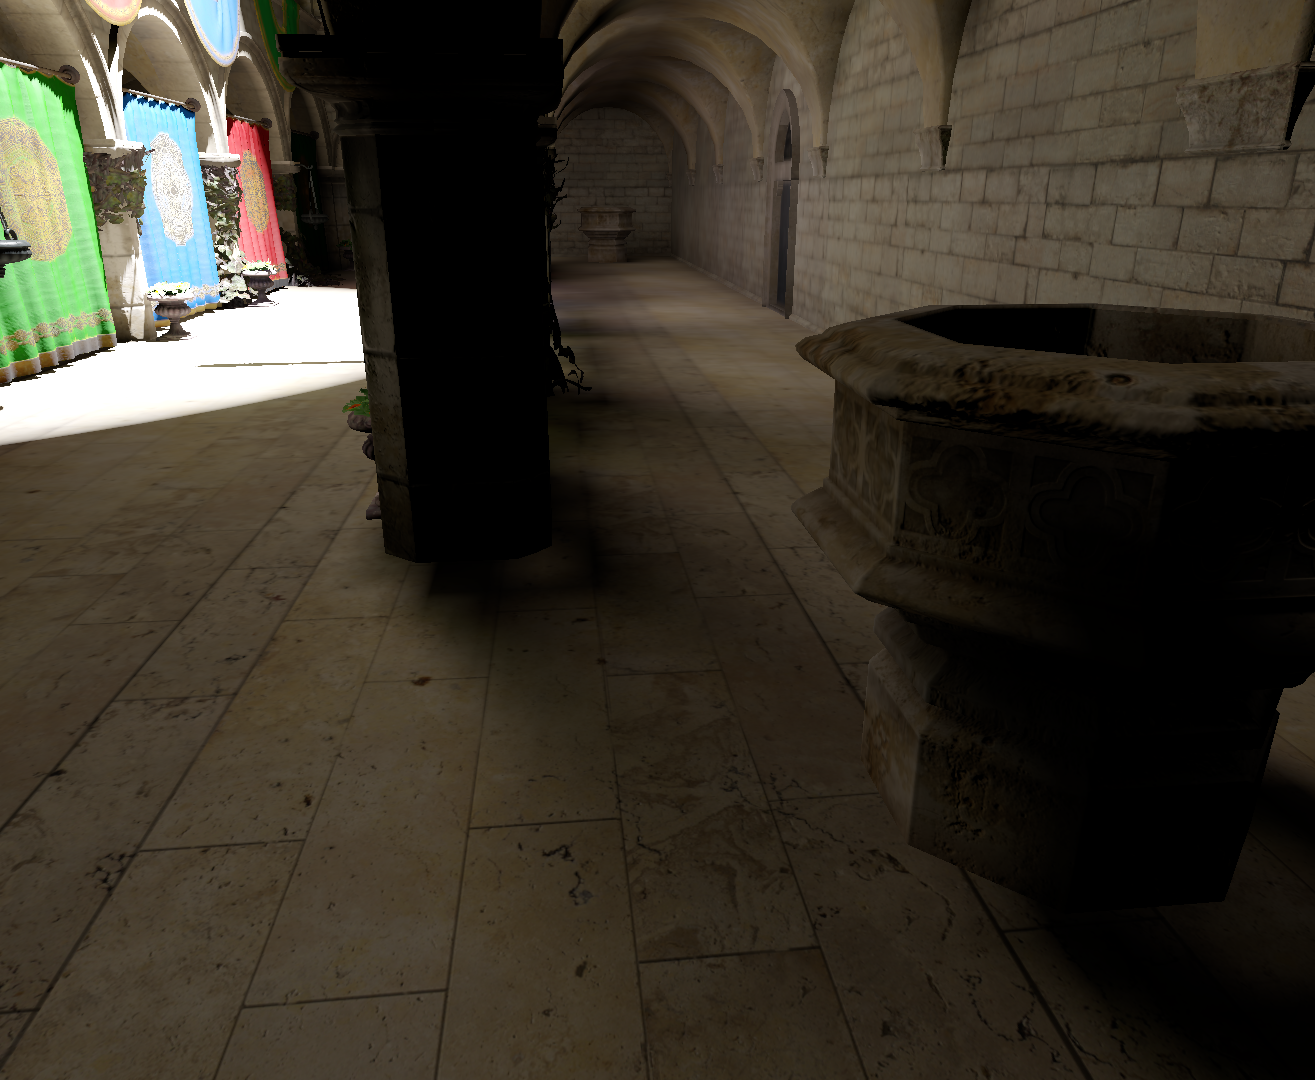
\includegraphics[width=\textwidth]{eva/shadow/vox256_cav64}
\caption{Voxelization: $256^3$ CAV: $4\times64^2$}
\end{subfigure}
\\
\begin{subfigure}[b]{\halfpageimage}
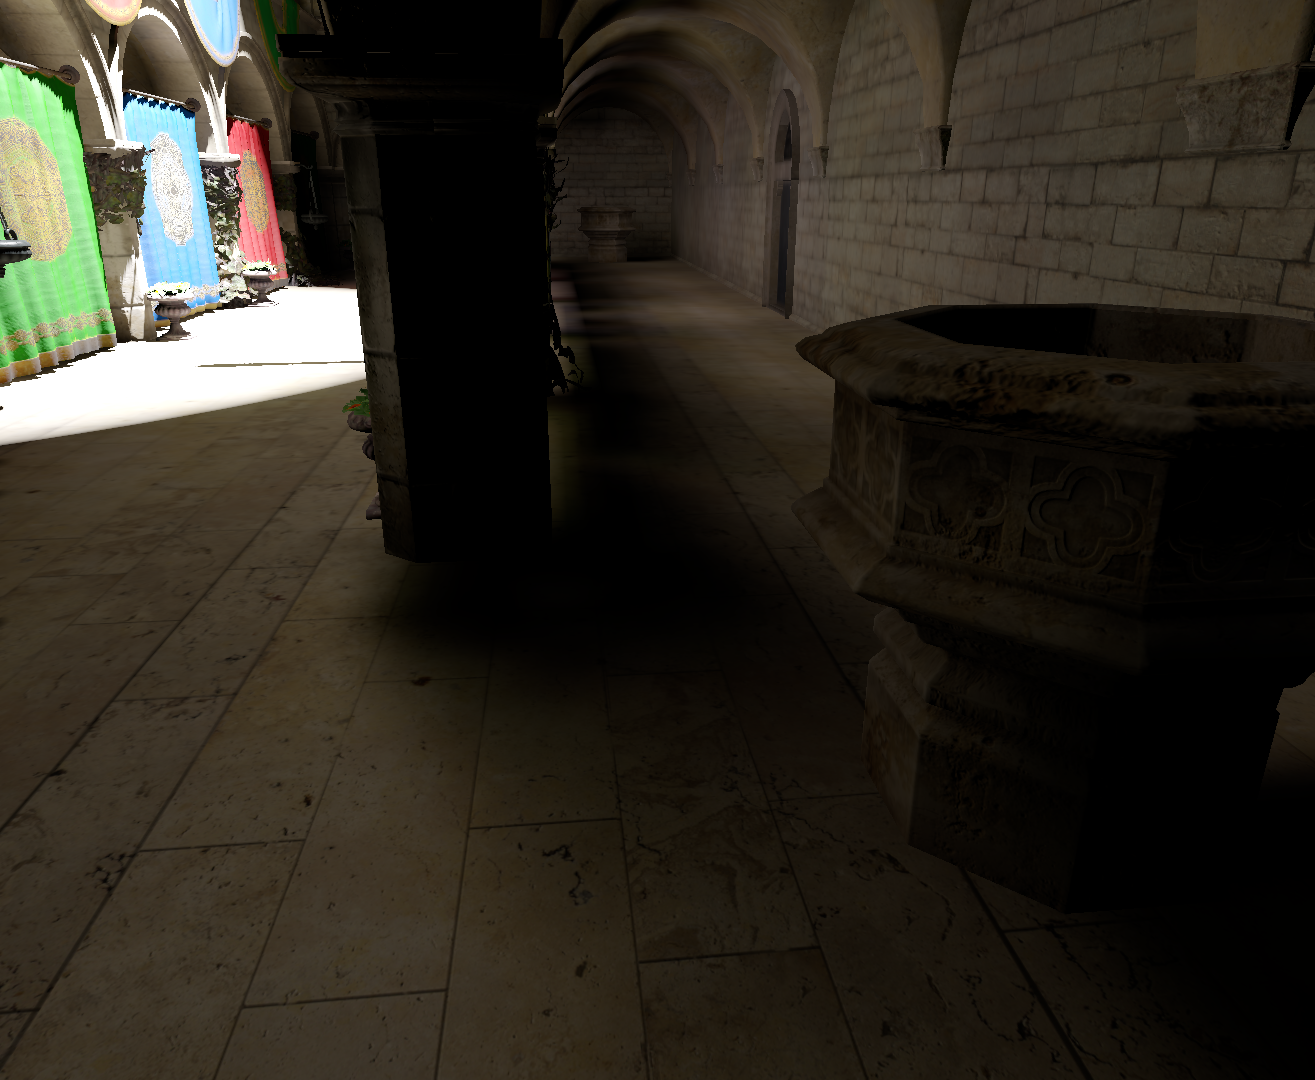
\includegraphics[width=\textwidth]{eva/shadow/vox128_cav128}
\caption{Voxelization: $128^3$ CAV: $4\times128^2$}
\end{subfigure}
\begin{subfigure}[b]{\halfpageimage}
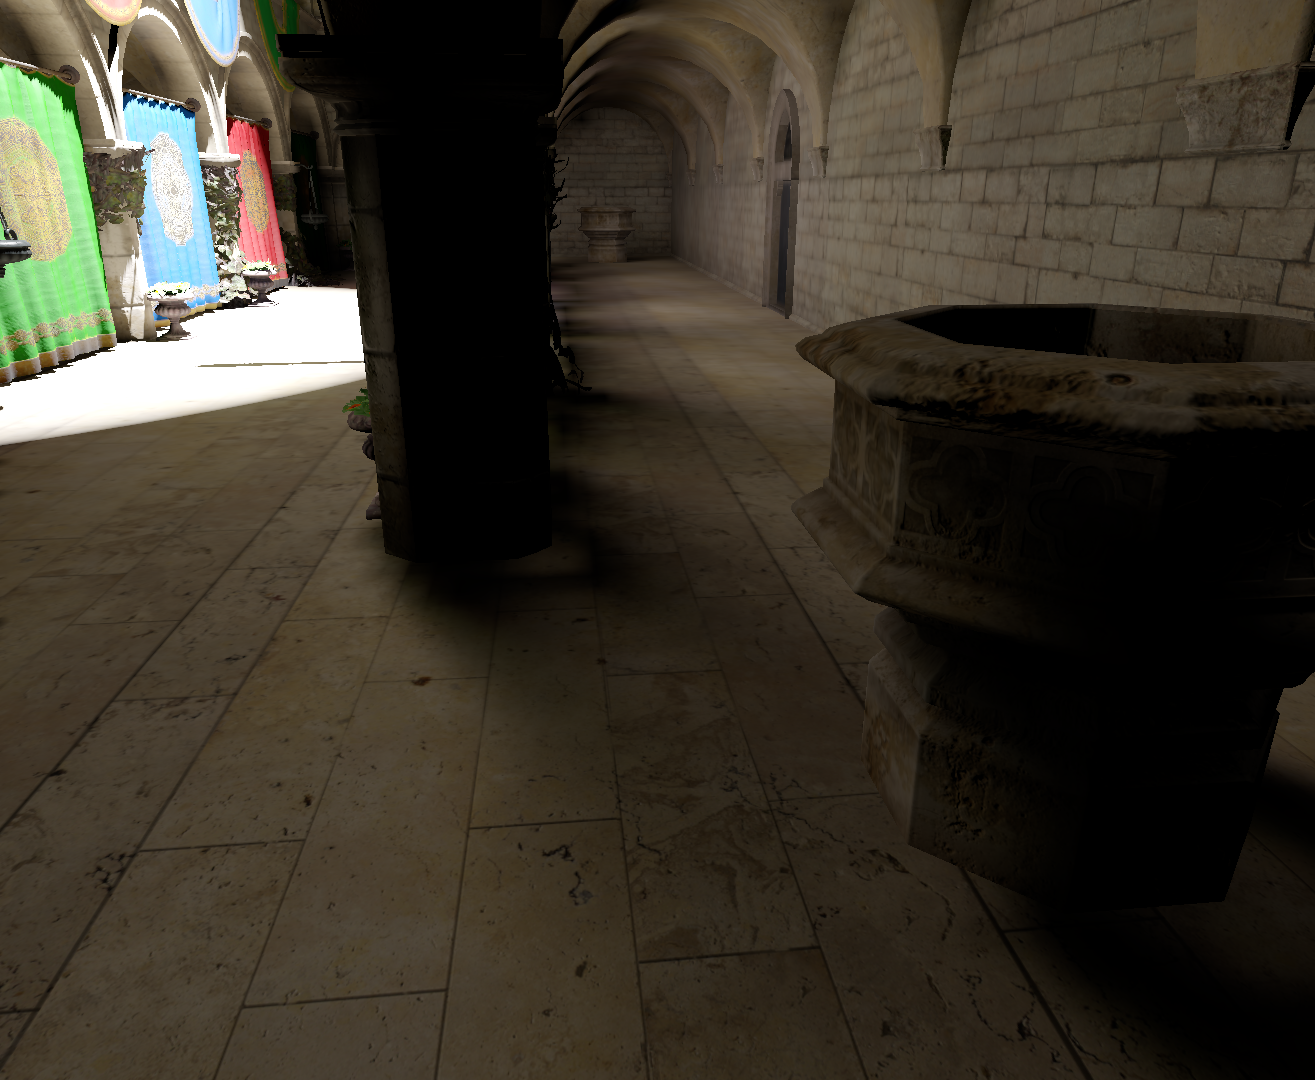
\includegraphics[width=\textwidth]{eva/shadow/vox256_cav128}
\caption{Voxelization: $256^3$ CAV: $4\times128^2$}
\end{subfigure}
\caption{Indirect shadow for different voxel volume and cascaded address volume resolutions in the \dataset{Sponza} scene.}
\label{fig:shadowcomparision:resolutions}
\end{figure}
%\todo{shadow images not bright enough}
%
\begin{figure}
\centering
\begin{subfigure}[b]{0.27\textwidth}
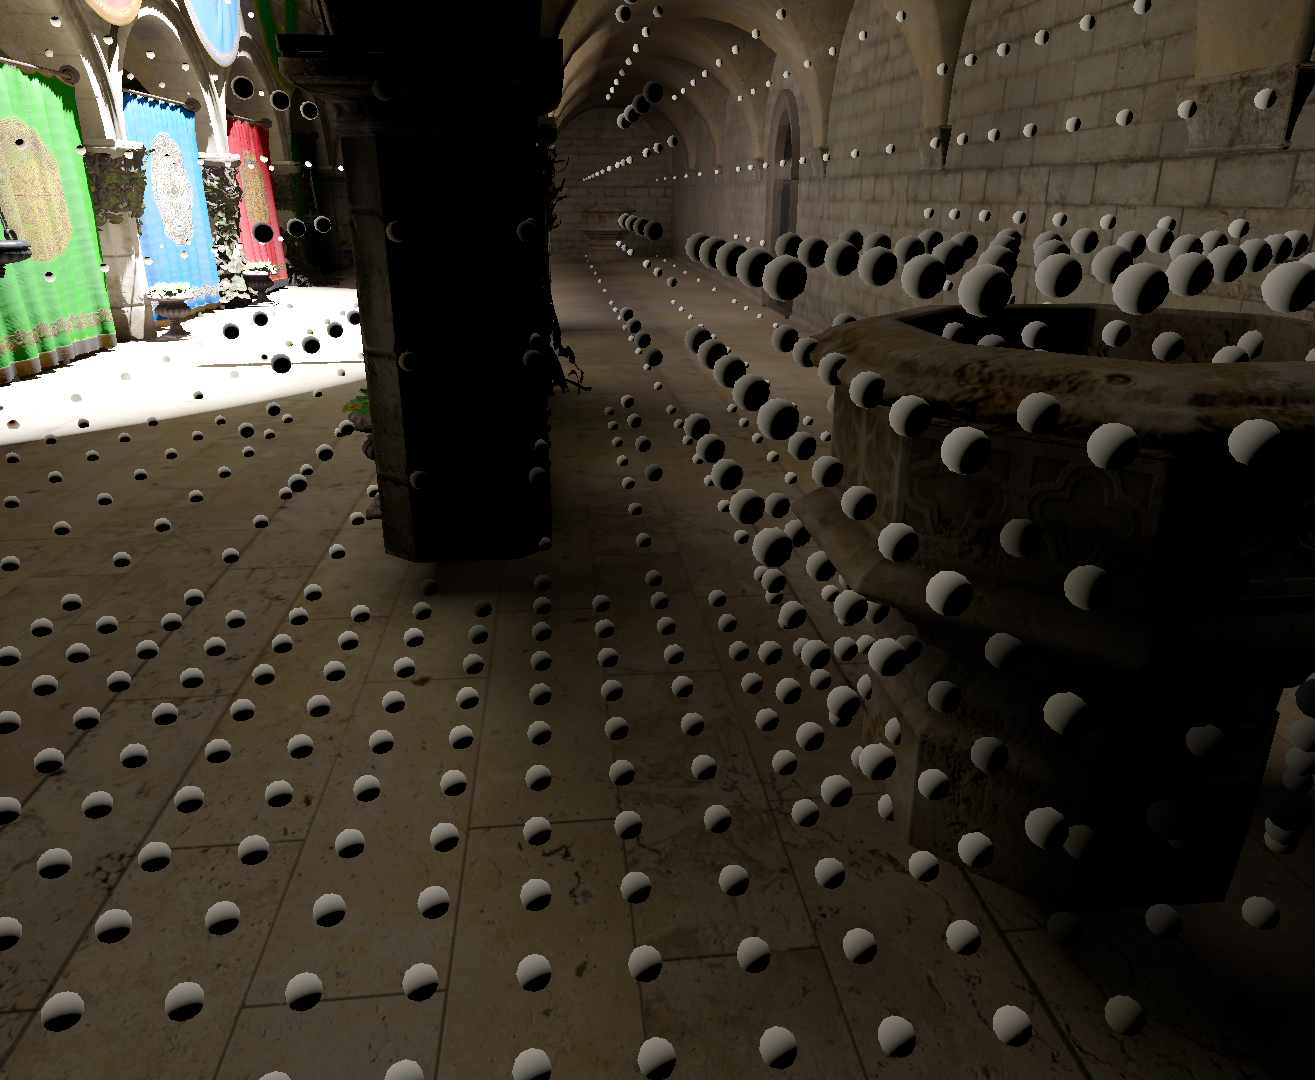
\includegraphics[width=\textwidth]{eva/shadow/vox256_cav32_cvis}
\caption{CAV: $4\times32^2$}
\end{subfigure}
\begin{subfigure}[b]{0.27\textwidth}
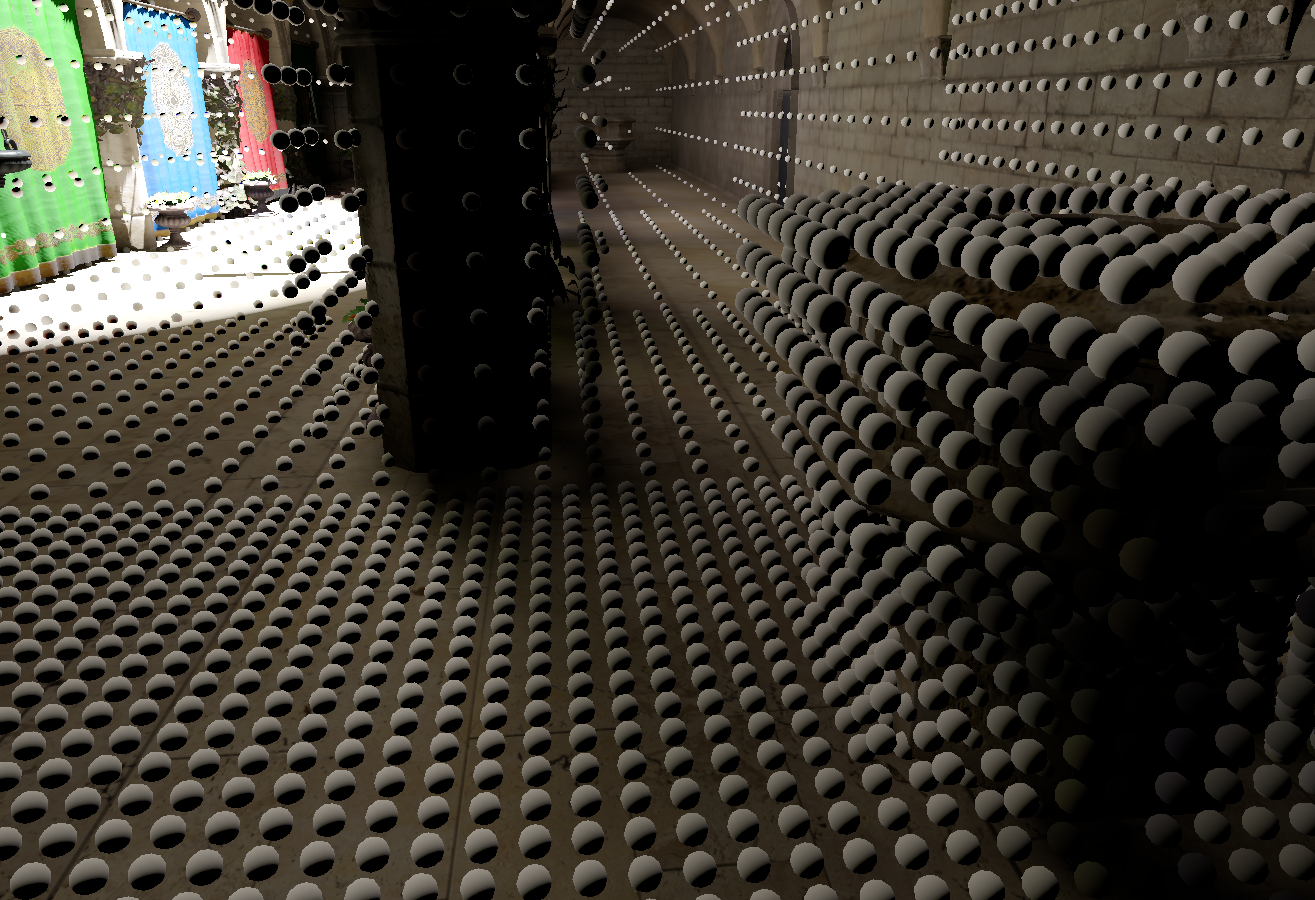
\includegraphics[width=\textwidth]{eva/shadow/vox256_cav64_cvis}
\caption{CAV: $4\times64^2$}
\end{subfigure}
\begin{subfigure}[b]{0.27\textwidth}
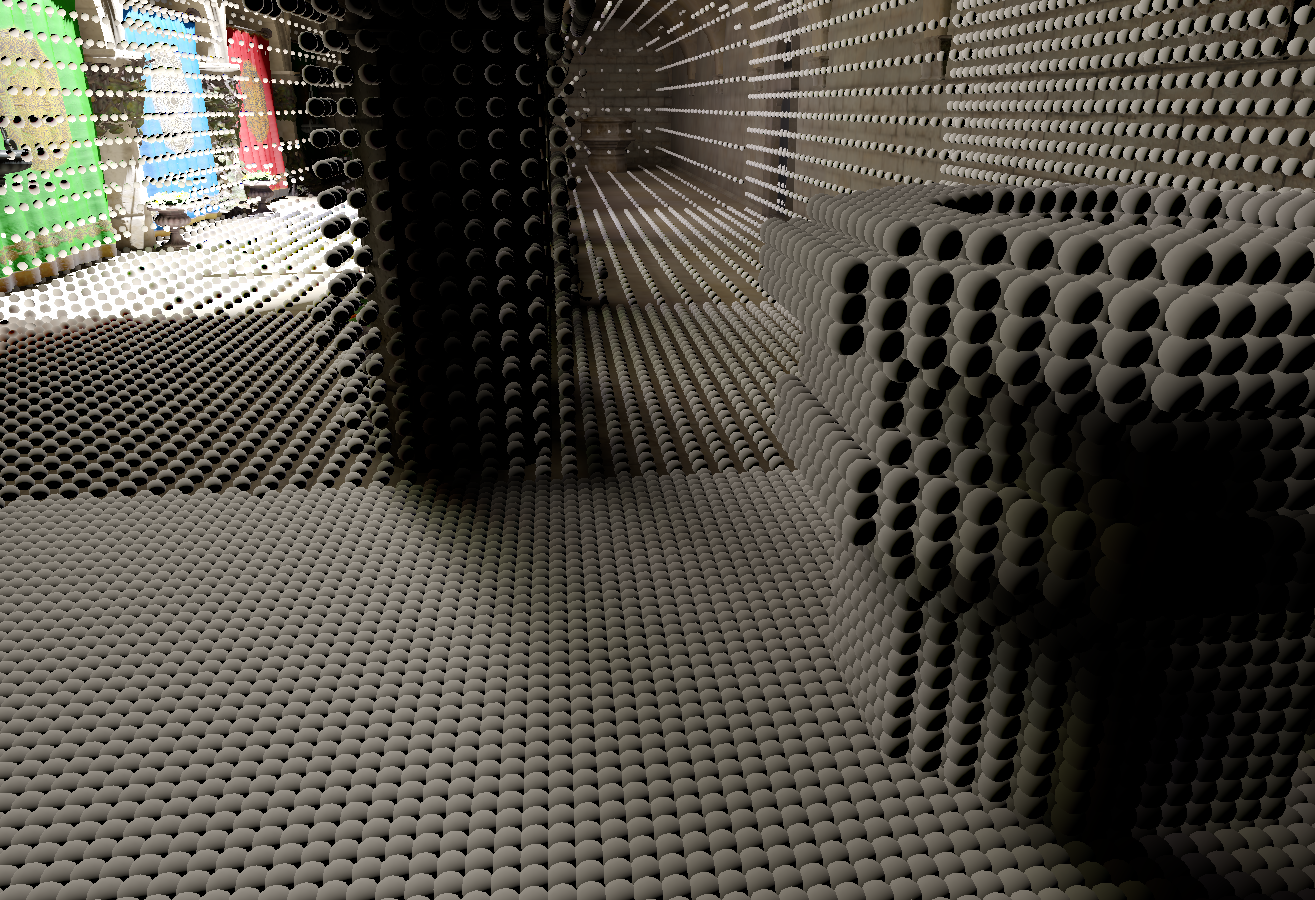
\includegraphics[width=\textwidth]{eva/shadow/vox256_cav128_cvis}
\caption{CAV: $4\times128^2$}
\end{subfigure}
\caption{Cache density visualization for \autoref{fig:shadowcomparision:resolutions}.}
\label{fig:shadowcomparision:resolutions:cavdensities}
\end{figure}
%
\begin{figure}
\begin{subfigure}[b]{\halfpageimage}
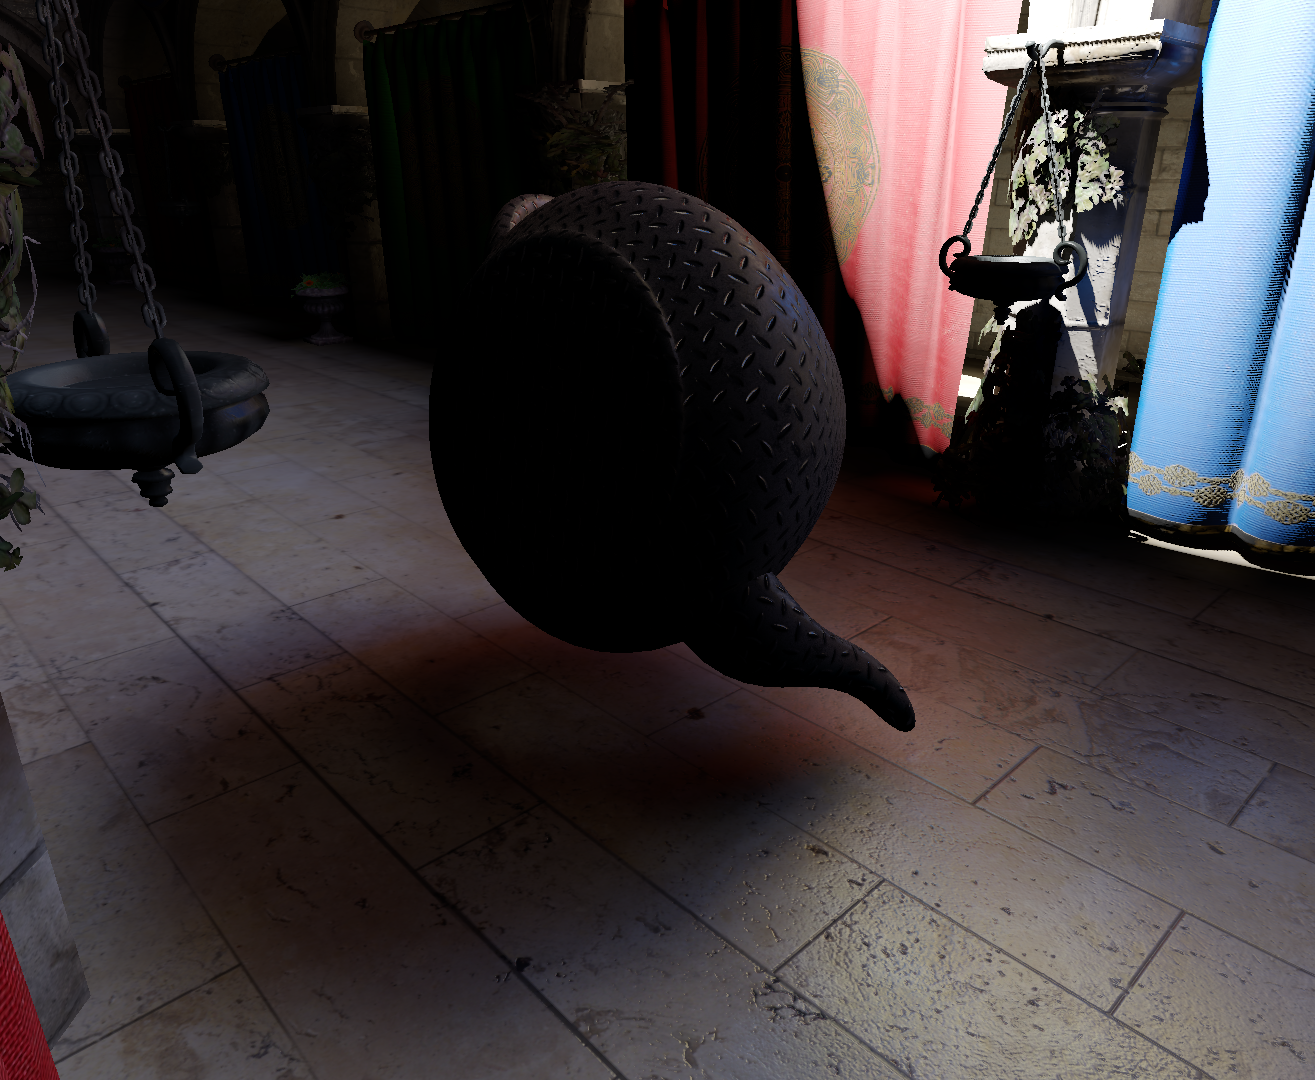
\includegraphics[width=\textwidth]{eva/shadow/lod0}
\caption{Shadow LOD 0}
\end{subfigure}
\begin{subfigure}[b]{\halfpageimage}
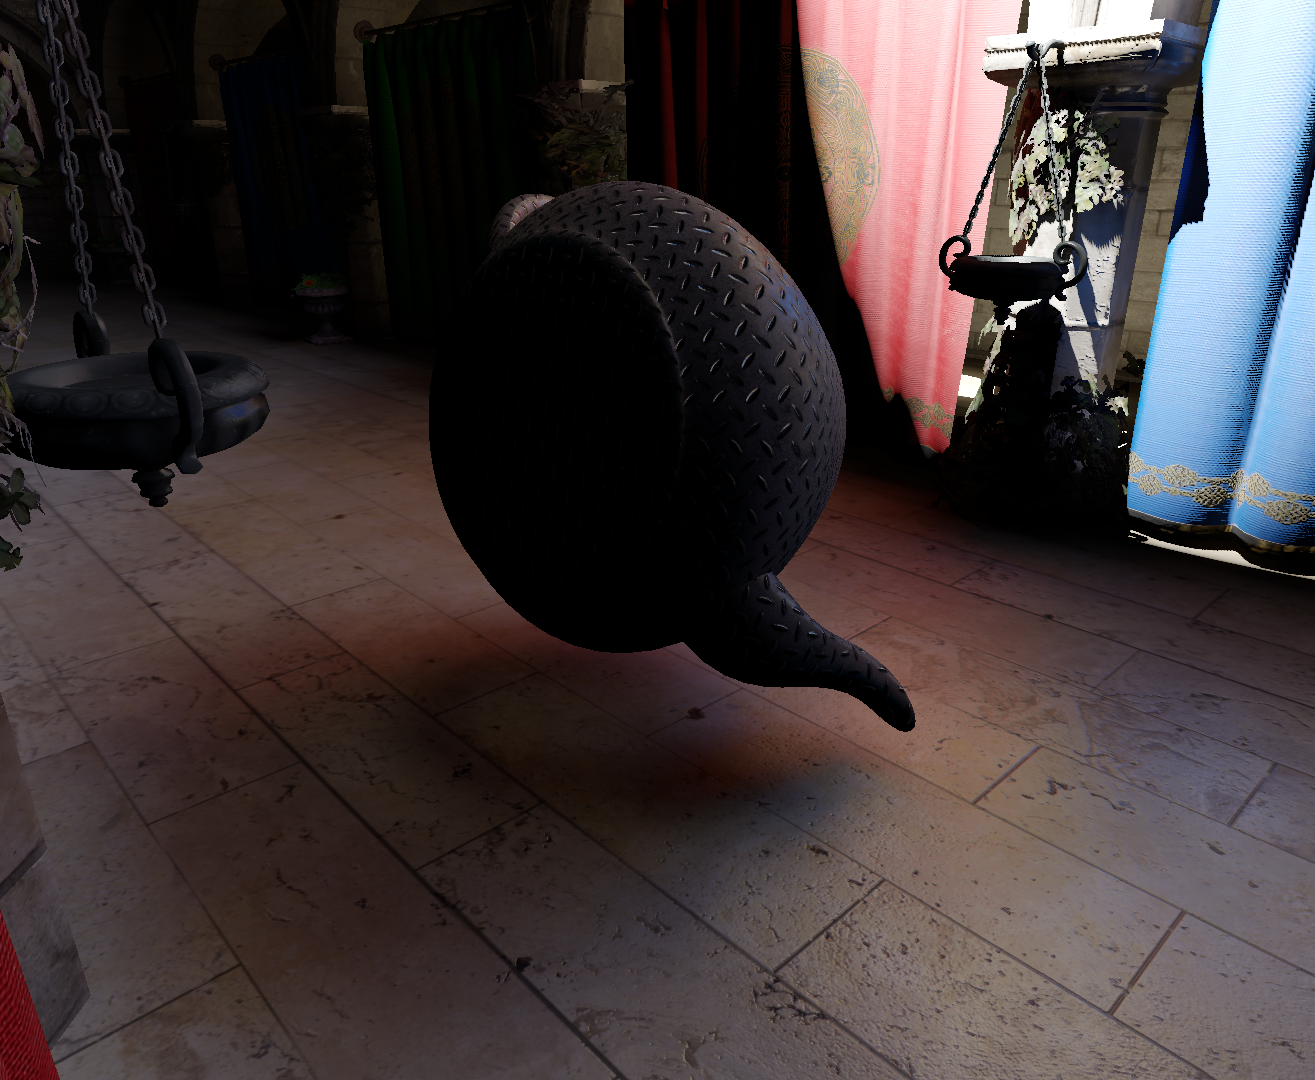
\includegraphics[width=\textwidth]{eva/shadow/lod1}
\caption{Shadow LOD 1}
\end{subfigure}
\\
\begin{subfigure}[b]{\halfpageimage}
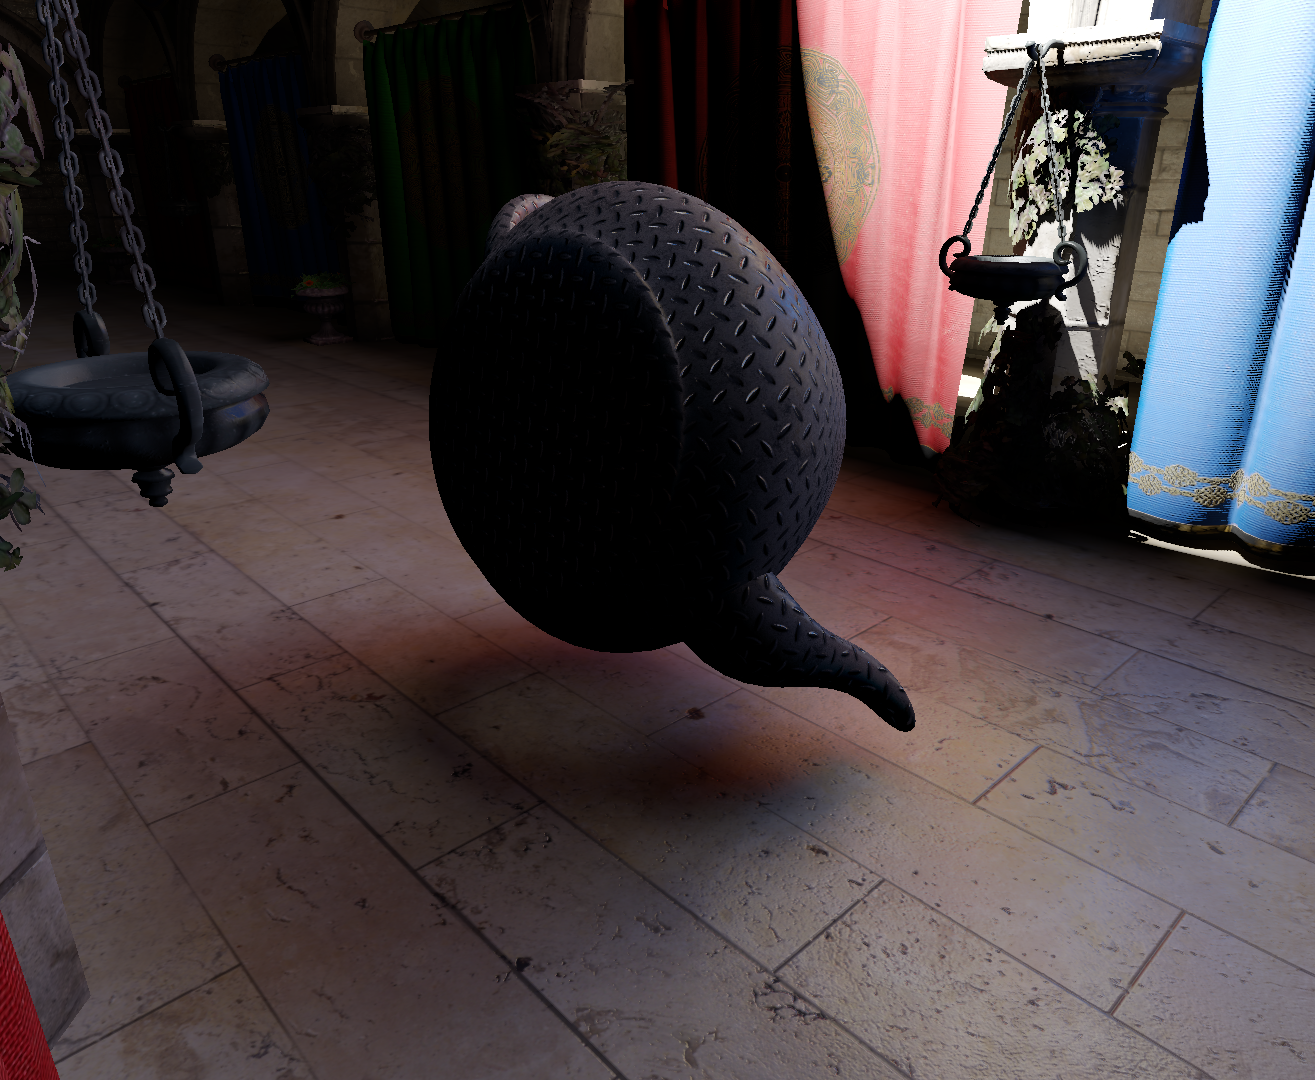
\includegraphics[width=\textwidth]{eva/shadow/lod2}
\caption{Shadow LOD 2}
\end{subfigure}
\begin{subfigure}[b]{\halfpageimage}
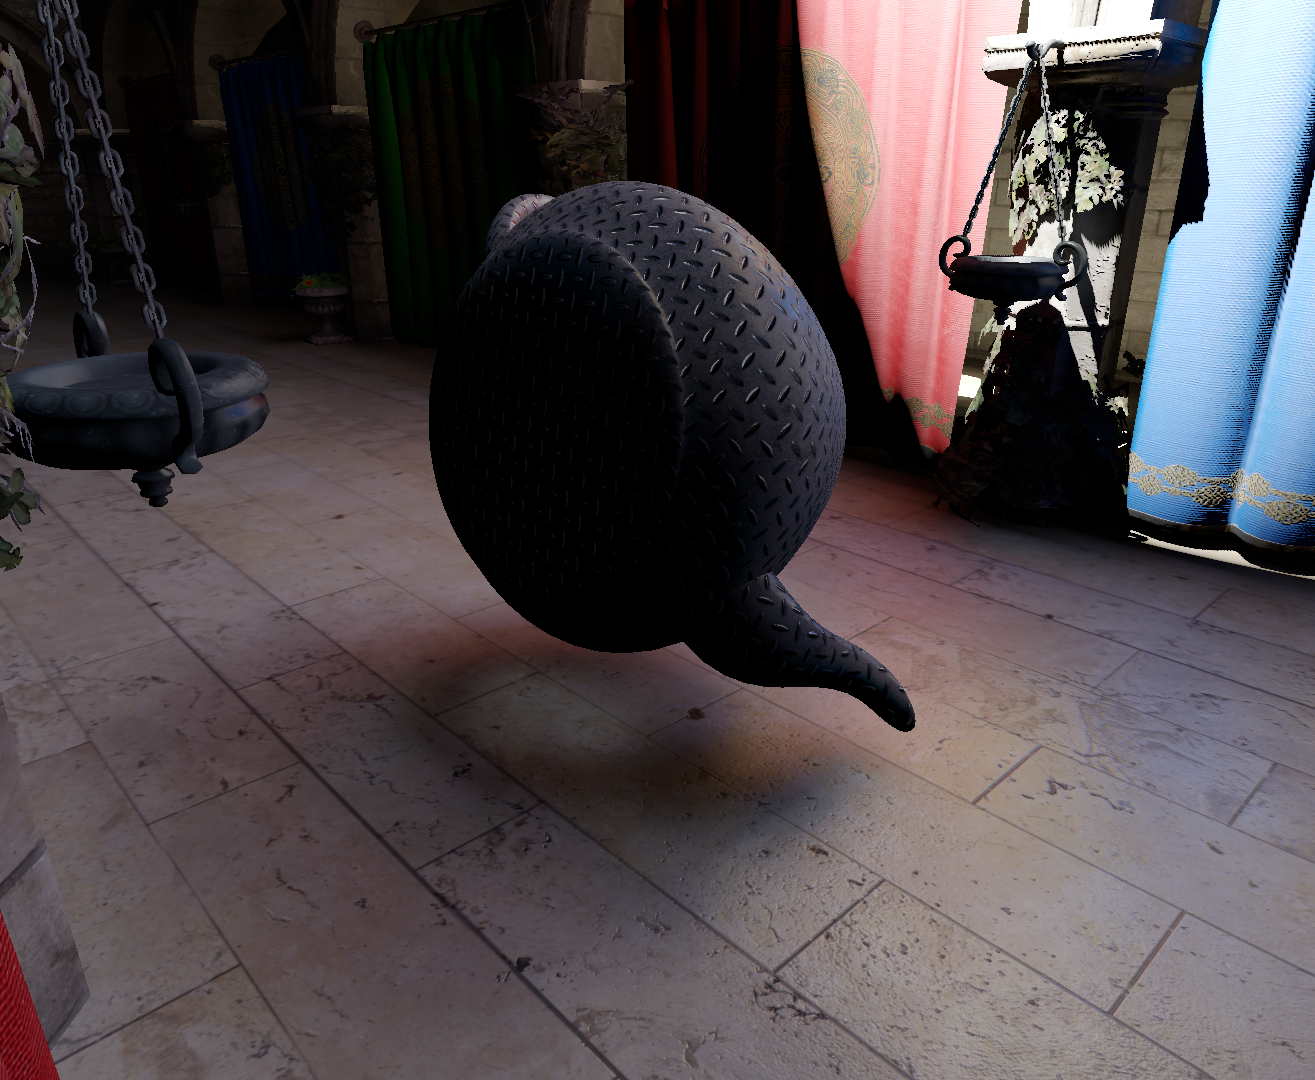
\includegraphics[width=\textwidth]{eva/shadow/lod3}
\caption{Shadow LOD 3}
\end{subfigure}
\\
\begin{subfigure}[b]{\halfpageimage}
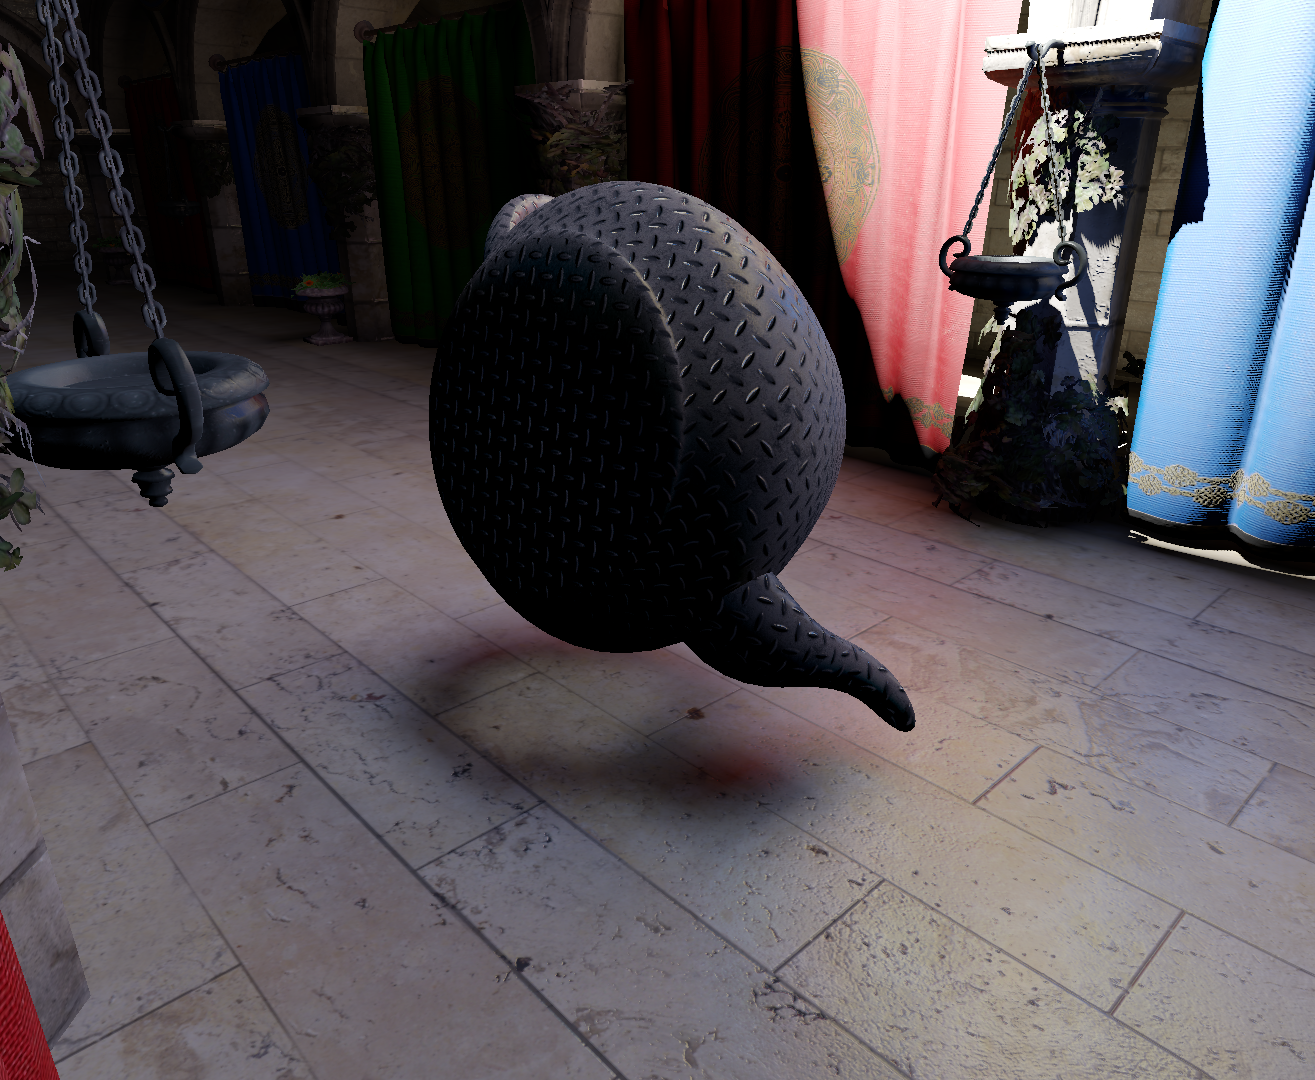
\includegraphics[width=\textwidth]{eva/shadow/lod4}
\caption{Shadow LOD 4}
\end{subfigure}
\begin{subfigure}[b]{\halfpageimage}
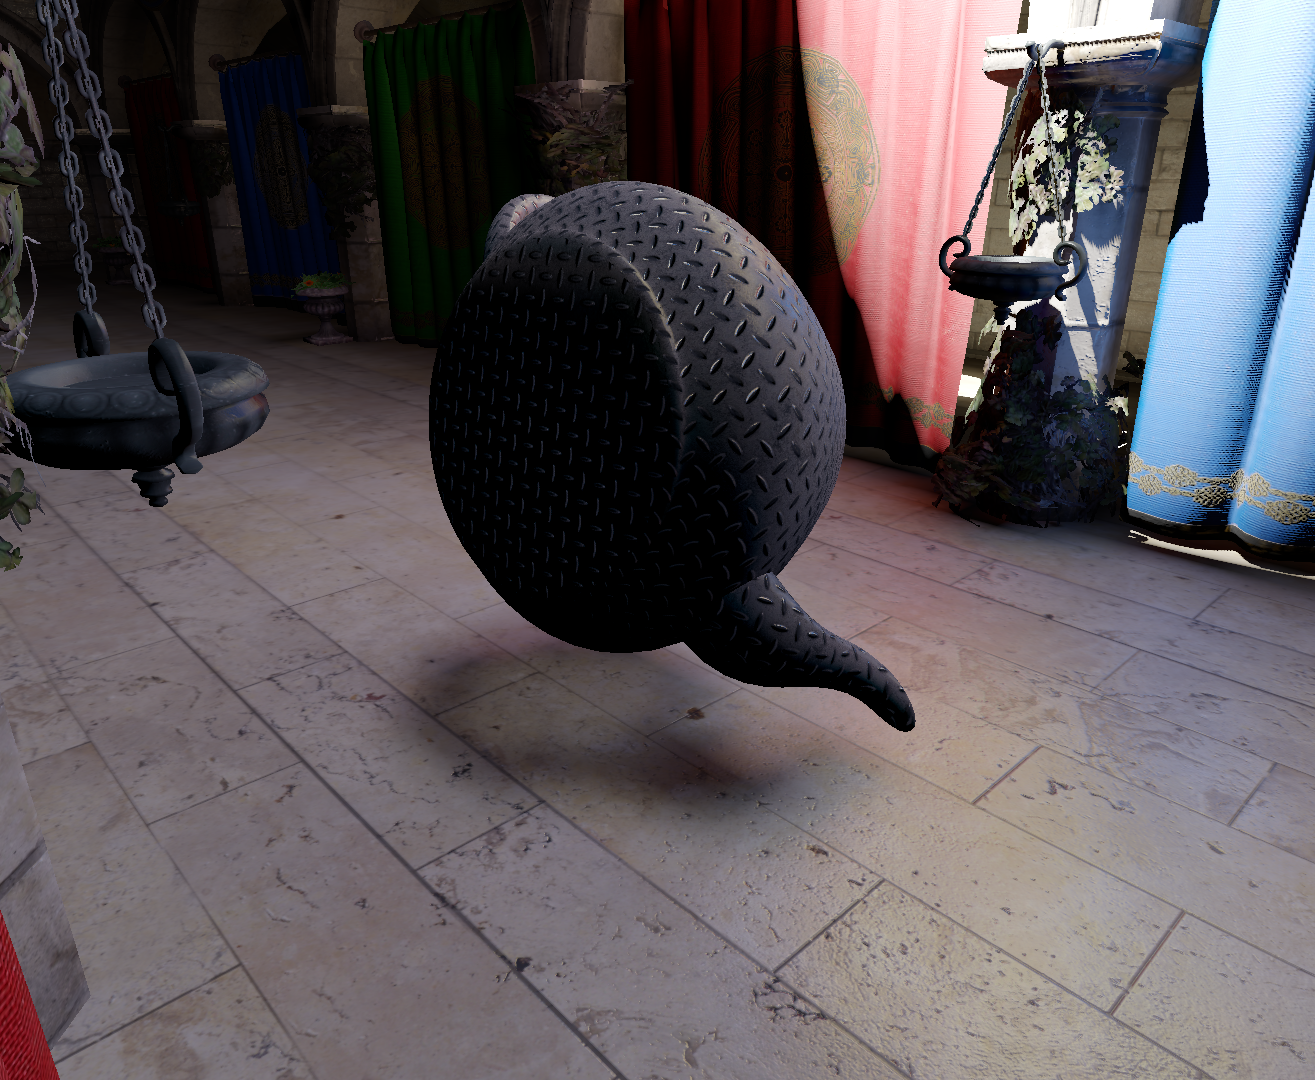
\includegraphics[width=\textwidth]{eva/shadow/lod5}
\caption{Shadow LOD 5}
\end{subfigure}
\caption{Indirect shadow for different shadow LODs in the \dataset{Sponza} scene using a voxel volume resolution of $256^3$ and CAV resolution of $64^3$. High LODs suffer from the low density in higher voxel mipmap levels which is the result of thin voxelization (as opposed to solid voxelization). }
\label{fig:shadowcomparision:lod}
\end{figure}
%

\subsection{Indirect Specular}\label{sec:eva:specquality}
As seen in \autoref{fig:specular:rescomparision}, the quality of indirect specular lighting seemingly improves straight-forward with higher specular environment map resolutions.
However, there are massive temporal coherence problems for resolutions beyond $16^2$ per cache.
The indirect specular lighting is the only part of our solution that has temporal coherency issues under camera movement, since the local hemispheres of the caches are view-dependent.
In combination with the single write each VAL performs per cache, this can result in flickering.
The effect is most problematic with high specular environment map resolutions.
As \autoref{fig:specular:cachegaps} shows, this leads to gaps on the specular environment map which are surrounded by too bright pixels since their samples should have been distributed into neighboring pixels as well.
We tried to close these gaps using a post-processing step similar as in imperfect shadow mapping \cite{bib:imperfectshadowmaps} but this did worsen temporal artifacts while not improving the visual quality noticeable.
However, for smaller resolutions the results are still visually pleasing and rather stable under movements.
%
\begin{figure}
\begin{subfigure}[b]{\halfpageimage}
\includegraphics[width=\textwidth]{eva/specular/0}
\caption{No indirect specular for comparison.}
\end{subfigure}
\begin{subfigure}[b]{\halfpageimage}
\includegraphics[width=\textwidth]{eva/specular/4}
\caption{specular environment map $4^2$}
\end{subfigure}
\\
\begin{subfigure}[b]{\halfpageimage}
\includegraphics[width=\textwidth]{eva/specular/8}
\caption{specular environment map $8^2$}
\end{subfigure}
\begin{subfigure}[b]{\halfpageimage}
\includegraphics[width=\textwidth]{eva/specular/16}
\caption{specular environment map $16^2$}
\end{subfigure}
\\
\begin{subfigure}[b]{\halfpageimage}
\includegraphics[width=\textwidth]{eva/specular/32}
\caption{specular environment map $32^2$}
\end{subfigure}
\begin{subfigure}[b]{\halfpageimage}
\includegraphics[width=\textwidth]{eva/specular/64}
\caption{specular environment map $64^2$}
\end{subfigure}
\caption{Indirect specular lighting for different specular environement map resolutions in the \dataset{Sponza} scene using CAV resolution of $64^3$. }
\label{fig:specular:rescomparision}
\end{figure}
\begin{figure}
\centering
\begin{subfigure}[b]{0.35\textwidth}
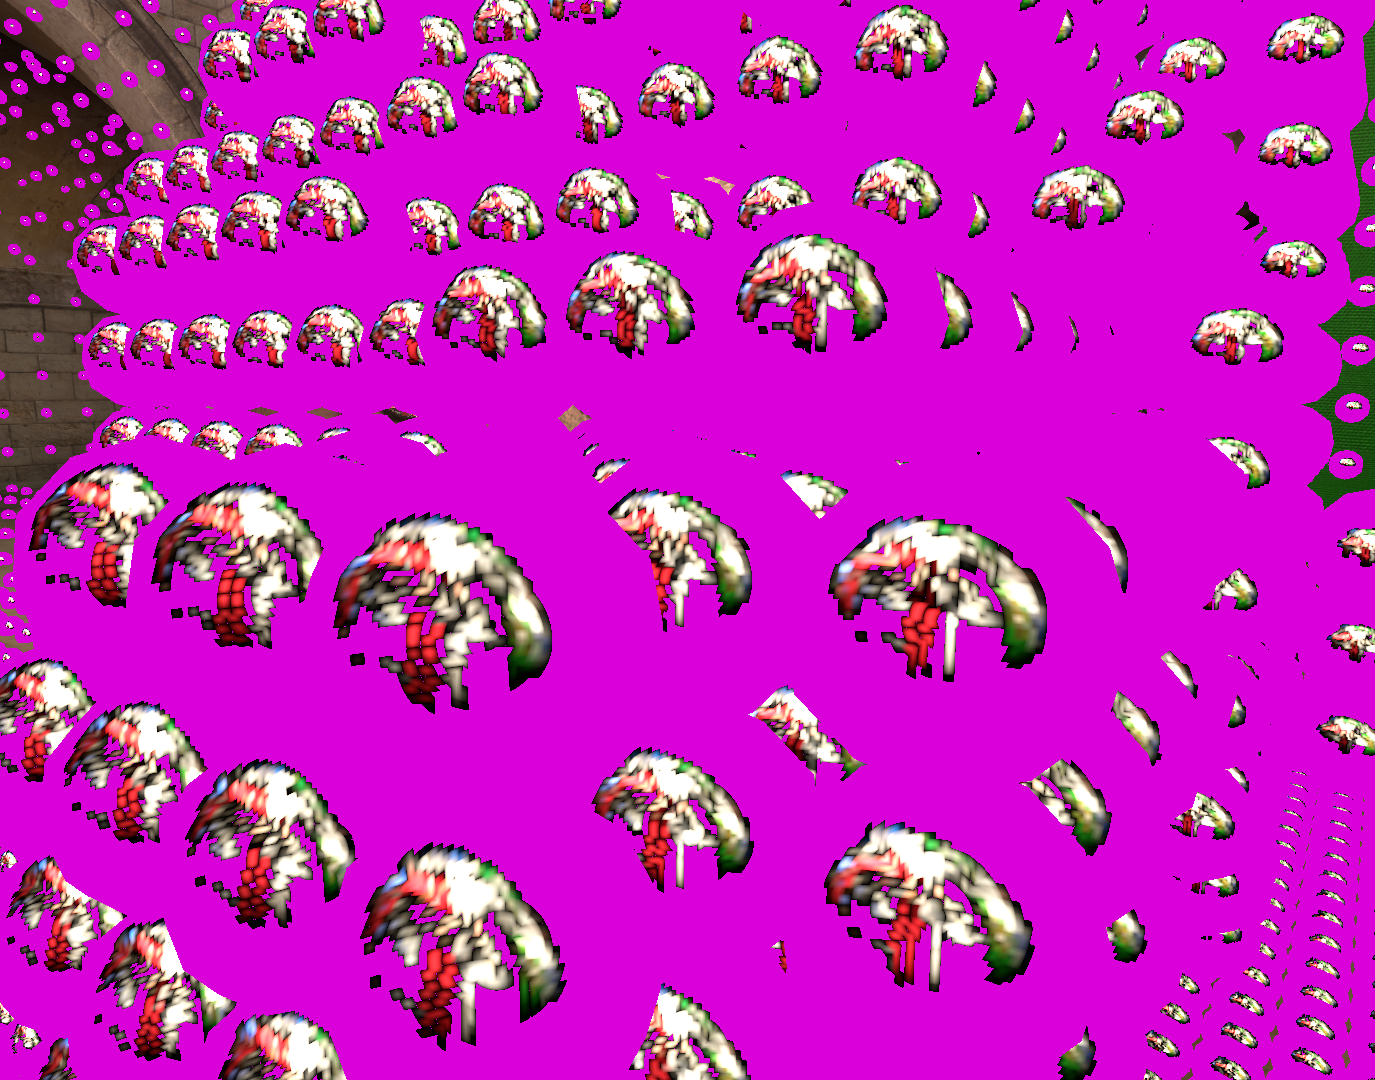
\includegraphics[width=\textwidth]{eva/specular/cache64_rsm64}
\caption{RSM resolution $64^2$.}
\end{subfigure}
\begin{subfigure}[b]{0.35\textwidth}
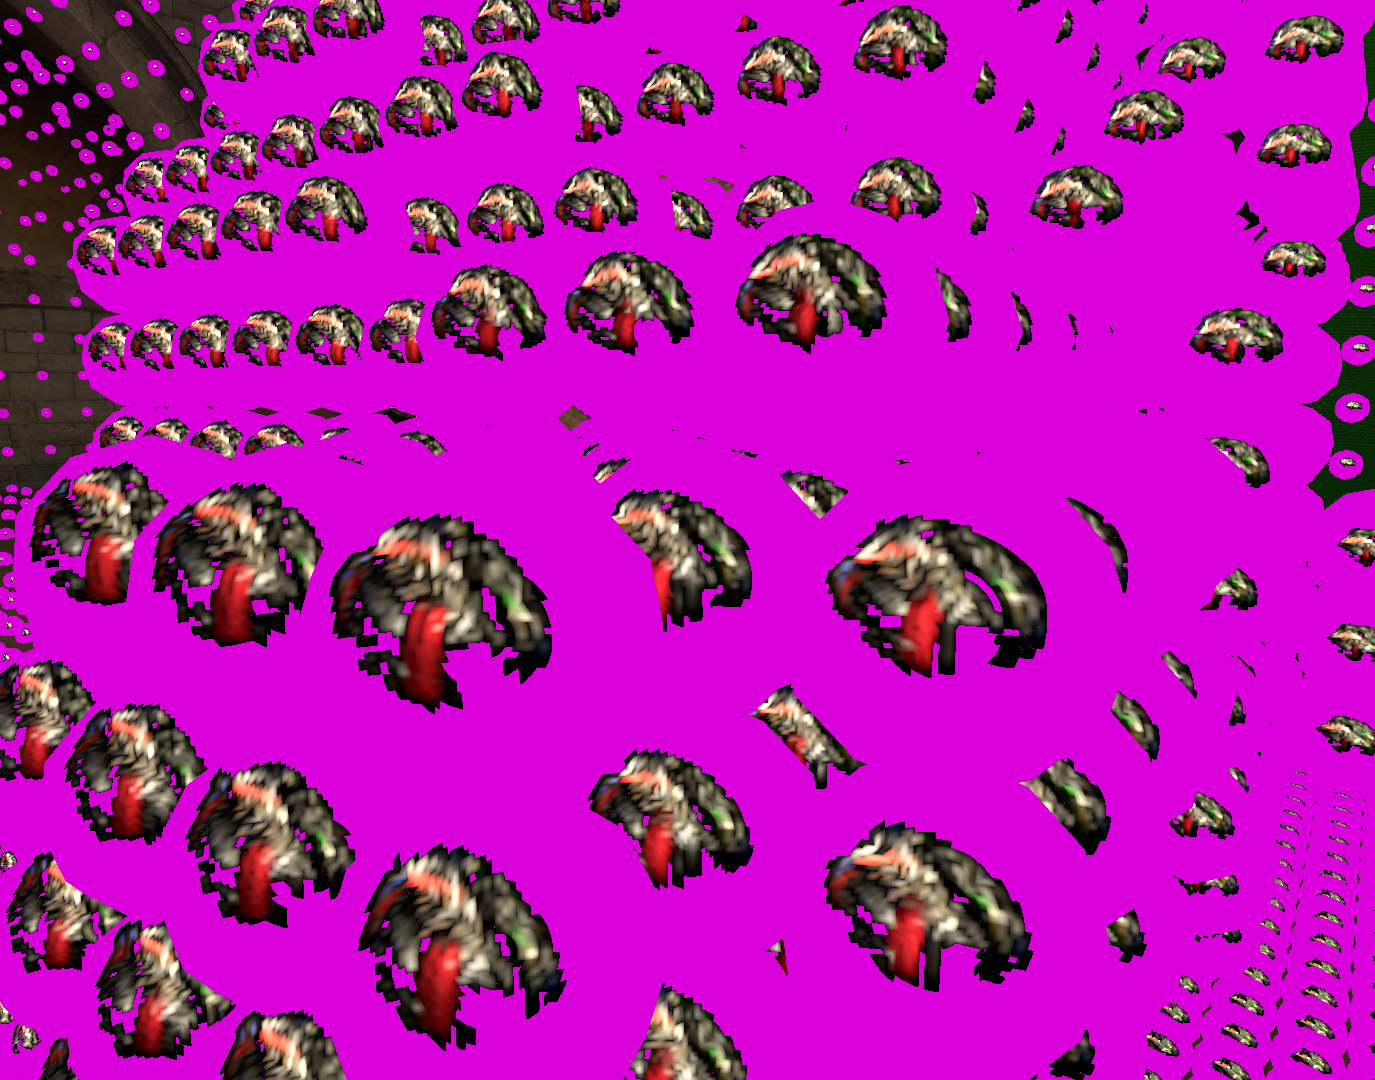
\includegraphics[width=\textwidth]{eva/specular/cache64_rsm256}
\caption{RSM resolution $256^2$}
\end{subfigure}
\caption{Specular environment map cache visualization in the teapot in \autoref{fig:specular:rescomparision}. Resolution of the specular environment map is $64^2$. Unwritten parts have been colored in magenta to highlight the gaps between samples. }
\label{fig:specular:cachegaps}
\end{figure}

\section{Memory Consumption} \label{sec:eva:memory}
\begin{table}[h]
\centering
\begin{tabular}{lrr}
\toprule
RSM & Flux + Depth + Normal & \SI{22.6}{\mebi\byte} \\
\hspace{0.5cm} \emph{Flux}   & $1024^2 \cdot \SI{6}{\byte} + \mathrm{mipmaps}$ & \textit{8.0\,MiB}\\ %\textit{\SI{8.0}{\mebi\byte}} \\
\hspace{0.5cm} \emph{Normal} & $1024^2 \cdot \SI{4}{\byte} + \mathrm{mipmaps}$ & \textit{5.3\,MiB}\\ %\textit{\SI{5.3}{\mebi\byte}} \\
\hspace{0.5cm} \emph{Depth + Depth}$^2$  & $1024^2 \cdot \SI{4}{\byte} + \mathrm{mipmaps}$ & \textit{5.0\,MiB}\\ %\SI{5.3}{\mebi\byte} \\
\hspace{0.5cm} \emph{Depth}  & $1024^2 \cdot \SI{4}{\byte}$ & \textit{4.0\,MiB}\\ %\SI{4}{\mebi\byte} \\
\midrule
CAV   & $4\times 32^3 \cdot \SI{4}{\byte}$ & \SI{0.5}{\mebi\byte} \\
\midrule
Voxel Volume & $128^3 \cdot \SI{1}{\byte} + \mathrm{mipmaps}$ & \SI{2.3}{\mebi\byte} \\
\midrule
Cache Buffer & $32768\times\mathrm{cache}$ & \SI{2.5}{\mebi\byte} \\
\hspace{0.5cm} \emph{Position (+ padding)} & $4 \cdot \SI{4}{\byte}$ & \textit{16\,B}\\ %\SI{16}{\byte} \\
\hspace{0.5cm} \emph{2 Band SH (3 colors)} & $16 \cdot \SI{4}{\byte}$ & \textit{64\,B}\\ %\SI{64}{\byte} \\
\midrule
SpecEnvMap &  $32768\times 16^2 \cdot \SI{4}{\byte}$ & \SI{32.0}{\mebi\byte} \\
\midrule
\midrule
\textbf{Overall} &       & \textbf{59.9\,MiB}\\ %\SI{59.9}{\mebi\byte} \\
\bottomrule
\end{tabular}
\caption{Memory consumption break-down of the default configuration with a maximum of about 32k caches.}
\label{tab:memory}
\end{table}
\autoref{tab:memory} shows a memory consumption break-down for the default sample configuration which was mentioned in \autoref{sec:eva:params}.
The RSM is responsible for a surprisingly large portion of the used space, since we start out with a rather high resolution and sample it down.
The flux texture consists of three half-floats, the normals are saved in two signed integers (encoding angles).
Further, two depth textures are needed:
One for holding both depth and squared depth which is used for the cache-lighting and another one which serves as depth buffer during the RSM rendering and as shadow map later on.
\\
The cascaded address volumes (CAV) consist of unsigned integers (\SI{4}{\byte}) that address caches in the cache buffer.
While the voxel volume has a rather high resolution and needs mipmaps, it is still far bellow the memory consumption of the RSM textures since each voxel needs only a single byte.
\\
The size of the cache buffer depends on the number of used SH bands (two: \SI{64}{\byte} three: \SI{112}{\byte}) and the number of reserved caches.
For this overview we assumed a maximum of 32768 caches, which is well beyond everything we measured.
It would also be possible to adjust this number during the rendering.
If indirect specular is activated, the maximum cache number plays a more important role since each cache needs an individual specular environment buffer (on the atlas).
With \SI{32}{\mebi\byte} this is the clearly the largest item in this configuration.

\section{Comparison to other Techniques} \label{sec:eva:comparisiontoother}
Exact comparisons to other real-time global illumination techniques are difficult since both quality and performance are often highly dependent on various implementation details.
To be able to make an appropriate attempt to address this issue, we would have needed to implement all techniques in an unified framework.
However, this is beyond the scope of this work.
\\
Therefore, we provide comparisons based only on theoretical facts and our personal estimates.
These are summarized in \autoref{tab:comparision}.
Diffuse indirections without shadows are generally handled well by all mentioned techniques which is why it is not listed in the table.

Indirect shadowing is comparatively accurate only with voxel cone tracing (VCT) \cite{bib:voxelconetracing} and our approach.
It is not handled at all by reflective shadow mapping (RSM) \cite{bib:reflectiveshadowmaps} and could possibly be much better in realtime radiance caching by Vardis et al. \cite{bib:radiancecachechromaticcompression} if more samples would be used.
\\
Indirect specular lighting is a major problem for all state-of-the-art global illumination techniques.
To our knowledge only VCT is able to accurately display glossy features with high specular exponents.
Our technique can provide moderate reflections but those have a disproportional effect on the performance.
Considering that LightSkin \cite{bib:LightskinPaper} handles the problem with very low data overhead using interpolated virtual lights, its results are surprisingly good.
RSM can handle the problem by brute force, evaluating the specular lighting for each virtual light in every pixel.
\\
Most techniques, including our own, cannot handle thin geometries well and show light bleeding artifacts.
\autoref{sec:fig:rsmbias} already discussed how to fix the typical "bright spot artifacts" of RSM.
Techniques with pre-computations like LightSkin can alleviate this problem, but may still suffer from missing detail for smaller features.
\\
With the exception of VCT, memory requirements are rarely a problem for the listed techniques.
Especially our technique is able to run on a very limited budget, as has been shown in the last section.


\begin{landscape}
\newcommand{\specialVspace}{\vspace{0.5cm}}

\begin{table}[h]
\centering
\begin{tabular}{llllll}
\toprule
Method  & \makecell[l]{Ind. shadows quality\\ \& basic approach} & \makecell[l]{Ind. specular freq.\\ \& basic approach} & Typical artifacts & \makecell[l]{Memory requ.\\ \& main bound} & Main perf. bound\\
\midrule

\specialVspace

Ours    & \makecell[l]{rather accurate\\cone traced (to RSM)}& \makecell[l]{medium \\ radiance hemispheres} & \makecell[l]{specular flickering \\ shadow jaggies, bleeding } & \makecell[l]{low\\spec. env. map} & \makecell[l]{shadow quality, \\ RSM resolution}\\

\specialVspace

\makecell[l]{Vardis et al. \\ \cite{bib:radiancecachechromaticcompression} } & \makecell[l]{coarse\\ray march in low-\\ res. occupancy volume} & \makecell[l]{low (theory)\\spherical harmonics} & light bleeding & \makecell[l]{medium\\SH bands, volumes} & \makecell[l]{volume resolution\\RSM sample count} \\

\specialVspace

\makecell[l]{LightSkin \\ \cite{bib:LightskinPaper}} & \makecell[l]{coarse, no color\\blocker estimates} & \makecell[l]{low\\similar to radiance cache\\encoded as virtual light} &  \makecell[l]{small features wrong \\ slight bleeding} & \makecell[l]{medium\\cache references} & cache count \\

\specialVspace

\makecell[l]{VCT \\ \cite{bib:voxelconetracing}} & \makecell[l]{rather accurate\\cone traced (in volume)} & \makecell[l]{high\\approx. with thin cone} & \makecell[l]{blocky reflections \\ bleeding} & \makecell[l]{high\\sparse voxel octree} & \makecell[l]{cone count\\ volume resolution} \\

\specialVspace

\makecell[l]{LPV \\ \cite{bib:lpt}} & \makecell[l]{very coarse\\injected blocker volume} & \makecell[l]{very low\\spherical harmonics} & \makecell[l]{heavy bleeding\\limited light range} & \makecell[l]{medium\\SH bands, volumes}  & \makecell[l]{volume resolution,\\SH bands} \\

\specialVspace

\makecell[l]{RSM \\ \cite{bib:reflectiveshadowmaps}} & n/a & \makecell[l]{arbitrary\\brute force} & \makecell[l]{bright splotches \\ ("fixable")} & \makecell[l]{very low\\RSM} & \makecell[l]{RSM resolution,\\sample-count per pixel}\\


\bottomrule
\end{tabular}
\caption{Coarse comparison of our technique with other realtime global illumination techniques. Except LightSkin \cite{bib:LightskinPaper}, all listed approaches work without any pre-computations.}
\label{tab:comparision}
\end{table}

\end{landscape}


\subfilebib % Makes bibliography available when compiling as subfile
\end{document}